\documentclass[paper=a5,pagesize=auto,twoside=false,fontsize=12pt,DIV=classic,BCOR=0mm,headinclude=true,footinclude=false]{scrbook}

%% font selection
\usepackage{utopia}
\usepackage{avant}

%% redefine headers
\usepackage[headsepline]{scrpage2}
\pagestyle{scrheadings}

\setkomafont{author}{%
  \normalfont\normalsize
}

\setkomafont{date}{%
  \normalfont\normalsize
}

\setkomafont{dedication}{%
  \raggedright\normalfont\small\itshape
}

\setkomafont{pageheadfoot}{%
  \normalfont\itshape
}

\automark[chapter]{chapter}
\renewcommand{\chaptermark}[1]{\markboth{#1}{#1}}
%\renewcommand{\sectionmark}[1]{\markright{#1}}

%% additional KOMA script options
\KOMAoptions{parskip=half,headsepline=true,numbers=noendperiod,captions=tableheading}
\recalctypearea{} % recalculate type area after selecting fonts

\usepackage{array}
\usepackage[british]{babel}
\usepackage{bbding}
\usepackage{fancyvrb}
\usepackage{float}  % direct positioning of floats
\usepackage{graphicx}
\usepackage{ifpdf}
\usepackage[utf8x]{inputenc}
\usepackage{paralist}
\usepackage{ucs}
\usepackage[obeyall]{siunitx}
\usepackage[hyphens,obeyspaces]{url}
\usepackage{varioref}
\usepackage{wrapfig}  % must be included after package "float"
\usepackage[dvipsnames]{xcolor}

%% Make sure "hyperref" comes last of your loaded packages, to give it
%% a fighting chance of not being over-written, since its job is to
%% redefine many LATEX commands.
\ifpdf
	\usepackage[unicode,pdftex]{hyperref}
\else
	\usepackage[unicode,hypertex]{hyperref}
\fi

\hypersetup{
  unicode=true,                % non-Latin characters in Acrobat’s bookmarks
  pdftitle=traKmeter,          % title
  pdfauthor=Martin Zuther,     % author
  pdfsubject=traKmeter,        % subject of the document
  pdfcreator=Martin Zuther,    % creator of the document
  colorlinks=true,             % false: boxed links; true: colored links
  linkcolor=blue,              % color of internal links
  citecolor=blue,              % color of links to bibliography
  filecolor=blue,              % color of file links
  urlcolor=blue                % color of external links
}

%% KOMA script captions
\addtokomafont{caption}{\small}
\addtokomafont{captionlabel}{\bfseries}
\setcapindent{0em}

%% taken from package "l2tabu"
\tolerance 1414
\hbadness 1414
\emergencystretch 1.5em
\hfuzz 0.3pt
\widowpenalty=10000
\vfuzz
\hfuzz
\raggedbottom

%% package "fancyvrb"
\DefineVerbatimEnvironment{VerbatimBoth}{Verbatim}{gobble=2,samepage=true,frame=single,framerule=0.4mm,framesep=2mm,xleftmargin=4mm,xrightmargin=4mm,rulecolor=\color{BurntOrange},label=32 and 64 bit}

\DefineVerbatimEnvironment{Verbatim32}{Verbatim}{gobble=2,samepage=true,frame=single,framerule=0.4mm,framesep=2mm,xleftmargin=4mm,xrightmargin=4mm,rulecolor=\color{OrangeRed},label=32 bit}

\DefineVerbatimEnvironment{Verbatim64}{Verbatim}{gobble=2,samepage=true,frame=single,framerule=0.4mm,framesep=2mm,xleftmargin=4mm,xrightmargin=4mm,rulecolor=\color{Cerulean},label=64 bit}

%% package "varioref"
\labelformat{chapter}{chapter~#1}
\labelformat{section}{section~#1}
\labelformat{subsection}{section~#1}
\labelformat{subsubsection}{section~#1}

\labelformat{figure}{figure~#1}
\labelformat{table}{table~#1}

%% package "paralist"
\setdefaultitem{\textbullet}{$\circ$}{}{}

%% package "url"
\urlstyle{rm}

%% package "wrapfig"
\setlength{\intextsep}{0.2\baselineskip}

%% package "siunitx"
\sisetup{per=slash,trapambigfrac,locale=UK}

\newunit[unitspace=space]{\dB}{dB}
\newunit[unitspace=space]{\dBFS}{dB\,FS}
\newunit[unitspace=space]{\dBSPL}{dB\,SPL}
\newunit[unitspace=space]{\dBu}{dBu}
\newunit[unitspace=space]{\LK}{LK}
\newunit[unitspace=space]{\LKFS}{LK\,FS}
\newunit[unitspace=space]{\VRMS}{V\textsubscript{RMS}}
\newunit[unitspace=space]{\VU}{VU}

%% scaling of screenshots
\newcommand{\screenshotscale}{0.7}

%% layout
\usepackage[inner=18mm,outer=18mm,top=26mm,bottom=27mm,headsep=6.5mm,headheight=5mm]{geometry}

% %% start new page for every section
% \let\stdsection\section  
% \renewcommand\section{\newpage\stdsection}

%% command "application"
\DeclareRobustCommand*{\application}[1]{\texttt{#1}}


%%% Local Variables:
%%% mode: latex
%%% mode: outline-minor
%%% TeX-command-default: "Rubber"
%%% TeX-master: "../trakmeter"
%%% TeX-PDF-mode: t
%%% ispell-local-dictionary: "british"
%%% End:

\input{include/hyphenation.sty}

\title{traKmeter}
\author{Martin Zuther}

\begin{document}

\title{traKmeter}

\subtitle{
  \normalsize{\textrm{\textmd{
        \vfill
        Loudness meter for correctly setting up \\
        tracking and mixing levels
        \vfill
        \vspace{1.5em}
        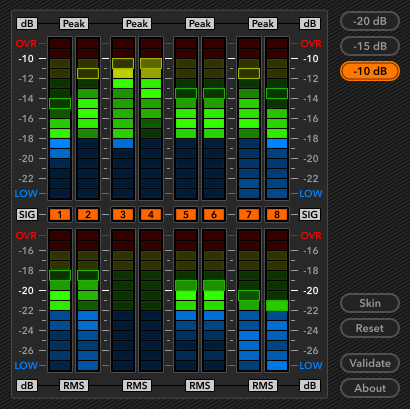
\includegraphics[scale=0.375,clip]{include/images/trakmeter.png}
        \vfill
      }}}
}

\author{}

\date{\emph{Last edited on \today}}

\dedication{
  
\includegraphics[scale=0.65,clip]{include/images/cc-by-sa.png}
  \vspace{0.25em}

  This documentation by \href{http://www.mzuther.de/}{Martin Zuther}
  is licensed under a
  \href{http://creativecommons.org/licenses/by-sa/4.0/}{Creative
    Commons Attribution-ShareAlike 4.0 International License} with the
  exception of trademark logos.

  \vspace{2.5em}

  
\includegraphics[scale=0.55,clip]{include/images/VST_Compatible_Logo_Steinberg_negative.png}

  VST is a trademark of Steinberg Media Technologies GmbH,
  registered in Europe and other countries.
}

\maketitle

\tableofcontents

\clearpage  % layout

\chapter{Digital recordings}
\label{chap:digital_recordings}

The digital revolution brought many advantages to the field of audio
processing: higher fidelity, less noise, non-degrading copies and the
endless possibilities of digital signal processing.  Unfortunately,
however, digital audio also introduced some problems of its own.

Whereas the analogue domain is relatively inert against very high
levels (overdriving some analogue equipment actually sounds pretty
good), the digital domain punishes even small transgressions into
forbidden territory with harsh clipping.

And while digital audio can be transferred without loss in quality, it
is degraded by each and every calculation, be it a simple change in
level, equalisation or a fancy effect.  Crossing domains from analogue
to digital and \emph{vice versa} leads to additional degradation.
Finally, changes in bit depth or sampling rate, jitter and
inter-sample peaks are nothing for the weak of heart.

However, most of these obstacles can easily be overcome by proper gain
staging, dithering, minimising the crossing of domains and choosing
appropriate bit depths and sampling rates right from the beginning.

If you carefully choose, test and operate your equipment, you're well
on your way to pure audio bliss \dots

\section{Definitions}
\label{sec:definitions}

\begin{tabular}{p{0.375 \textwidth}p{0.525 \textwidth}}

  \textbf{RMS} \newline
  \emph{root mean square} &
  statistical method used for calculating an average from fluctuating
  values \\[0.5em]

  \textbf{\si{\dBu}} \newline
  \emph{decibel unterminated} &
  level ratio with an analogue reference level of \SI{0.7746}{\VRMS}
  \\[0.5em]

  \textbf{\si{\dBFS}} \newline
  \emph{decibel relative to \newline digital full-scale} &
  level ratio with a reference level equal to the maximum
  representable value of a digital signal \\[0.5em]

  \textbf{\si{\dBr}} \newline
  \emph{decibel relative to \newline reference level} &
  level ratio with an arbitrary reference level that must be specified;
  for instance, \SI{0}{\dBr} may be equal to \SI{-20}{\dBFS} \\[0.25em]

\end{tabular}

\section{Gain staging}
\label{sec:gain_staging}

The process of setting audio devices to run at optimal input and
output levels is called \emph{gain staging}.

Professional analogue audio equipment is designed to be run at a
nominal level of \SI[retain-explicit-plus]{+4}{\dBu}.  This leaves a
headroom for peaks of at least \textbf{\SI{20}{\dB}} to the clipping
point.  Thus, driving all analogue audio equipment at
\SI[retain-explicit-plus]{+4}{\dBu} ensures an optimal signal-to-noise
ratio while preventing clipping and keeping all transients intact.

Now let's transfer this to the digital domain.  First, choose an
analogue reference level for your converter.\footnote{for more
  information, see
  \href{https://www.digido.com/portfolio-item/level-practices-part-1/}{Level
    Practices (Part 1)} by Bob Katz; a reference level of
  \SI[retain-explicit-plus]{+4}{\dBu} = \SI{-15}{\dBFS} works well for
  me} Then, record with an average input level of
\textbf{\SI{-20}{\dBFS} RMS}.  Again, this ensures a good
signal-to-noise ratio while preventing clipping.  In addition, this
level drives your outboard equipment and most of your plug-ins at
their ``sweet spot''.

I also recommend recording with a maximum level of
\textbf{\SI{-10}{\dBFS} peak}.  This will leave enough space for
sudden jumps in level and may also improve the sound of your
recordings.  Some analogue-to-digital converters already degrade audio
when fed with levels close to digital full-scale (\SI{0}{\dBFS}),
resulting in the ``harshness'' that is often attributed to digital
audio.

\emph{Try this: record a clearly defined signal (such as a sine wave)
  and increase its level while analysing the obtained signal with a
  spectrum meter.  Overtones will probably appear at levels way below
  clipping point (see \ref{sec:converter_clipping}).  Their individual
  level may be low but will accumulate when you mix recordings -- and
  our ears are sensitive for distortion.}

Gain staging doesn't stop here.  Set up your mixer so that channel
levels are lower than subgroup levels, which in turn should be lower
than the master output levels.  No clipping should occur anywhere in
the mixer, which is especially important if you want to insert
external analogue gear.\footnote{for mixer inserts, I recommend
  maximum input and output levels of \textbf{\SI{-10}{\dBFS} peak} for
  the same reasons mentioned above} Do not overload effects or
plug-ins and (if possible) try to match their input and output
volume.\footnote{many digital signal processors use floating-point
  calculations and handle clipping gracefully; others, especially
  those modelling old analogue equipment, may clip badly}

Speaking of me, once I transitioned to proper gain staging, my
recordings and mixes became much cleaner.  And the effort involved was
pretty small!

\section{Digital audio myths}
\label{sec:digital_audio_myths}

I can almost hear you: digital recordings should be made at peak
levels close to but not exceeding \SI{0}{\dBFS}.  Unfortunately, this
misleading information has ended up in many manuals for professional
audio equipment.  But that doesn't make it any truer \dots

Even if you record at \emph{peak} levels of \SI{-18}{\dBFS}, a bit
depth of \SI{16}{\bits} will yield a signal-to-noise ratio of
\SI{78}{\dB}.  That is about what you can expect from the best
professional analogue tape machines and recording desks!

But think of the approximate \SI{19}{\bits} modern converters can
capture.\footnote{all real-world analogue circuits are contaminated
  with thermal noise which limits the achievable signal-to-noise ratio
  of converters} In this case, recording at peak levels of
\SI{-18}{\dBFS} yields an incredible signal-to-noise ratio of
\SI{96}{\dB}.  This is \emph{fully equivalent} to using a bit depth of
\SI{16}{\bits} and recording at levels close to clipping point!

\textbf{So there really is no point in recording at extreme levels.}

If you are still sceptical, read these three Gearslutz posts written
by a renowned engineer:
\href{https://www.gearslutz.com/board/showpost.php?p=10739624&postcount=9}{\#1},
\href{https://www.gearslutz.com/board/showpost.php?p=5063154&postcount=219}{\#2}
and
\href{https://www.gearslutz.com/board/showpost.php?p=9909382&postcount=96}{\#3}.
The highly regarded manufacturer \emph{Harrison Audio} also recommends
a maximum peak recording level of
\href{http://www.harrisonconsoles.com/mixbus/mixbus32c-6-live-manual/1/en/topic/gain-staging}{\SI{-15}{\dBFS}}
for their \emph{Mixbus 32C} digital audio workstation.  Finally, I
highly recommend reading
\href{https://www.soundonsound.com/techniques/gain-staging-your-daw-software}{this article}
in \emph{Sound On Sound}.

\section{Introducing traKmeter}
\label{sec:introducing_trakmeter}

Sadly, most digital audio equipment only has peak meters.  This is
readily understandable as you want to avoid digital clippings by all
means.  However, badly chosen meter ranges and scales often render
these meters useless.  And the lack of average meters does not exactly
facilitate gain staging.

When I had realised this, I started coding traKmeter.  It has evolved
with my growing knowledge and recording experience, but the underlying
ideas haven't changed at all.

\section{Converter clipping}
\label{sec:converter_clipping}

This experiment was conducted with a \emph{RME Fireface 800} interface
(\SI{96}{\kilo\hertz}, 24 bits, \SI{0}{\dBFS} set to
\SI[retain-explicit-plus]{+19}{\dBu}).  Signals were sent to an output
connected directly to an input (\textbf{red lines}).  A floating input
served as reference (\textbf{blue lines}).

\subsection{Single sine wave}

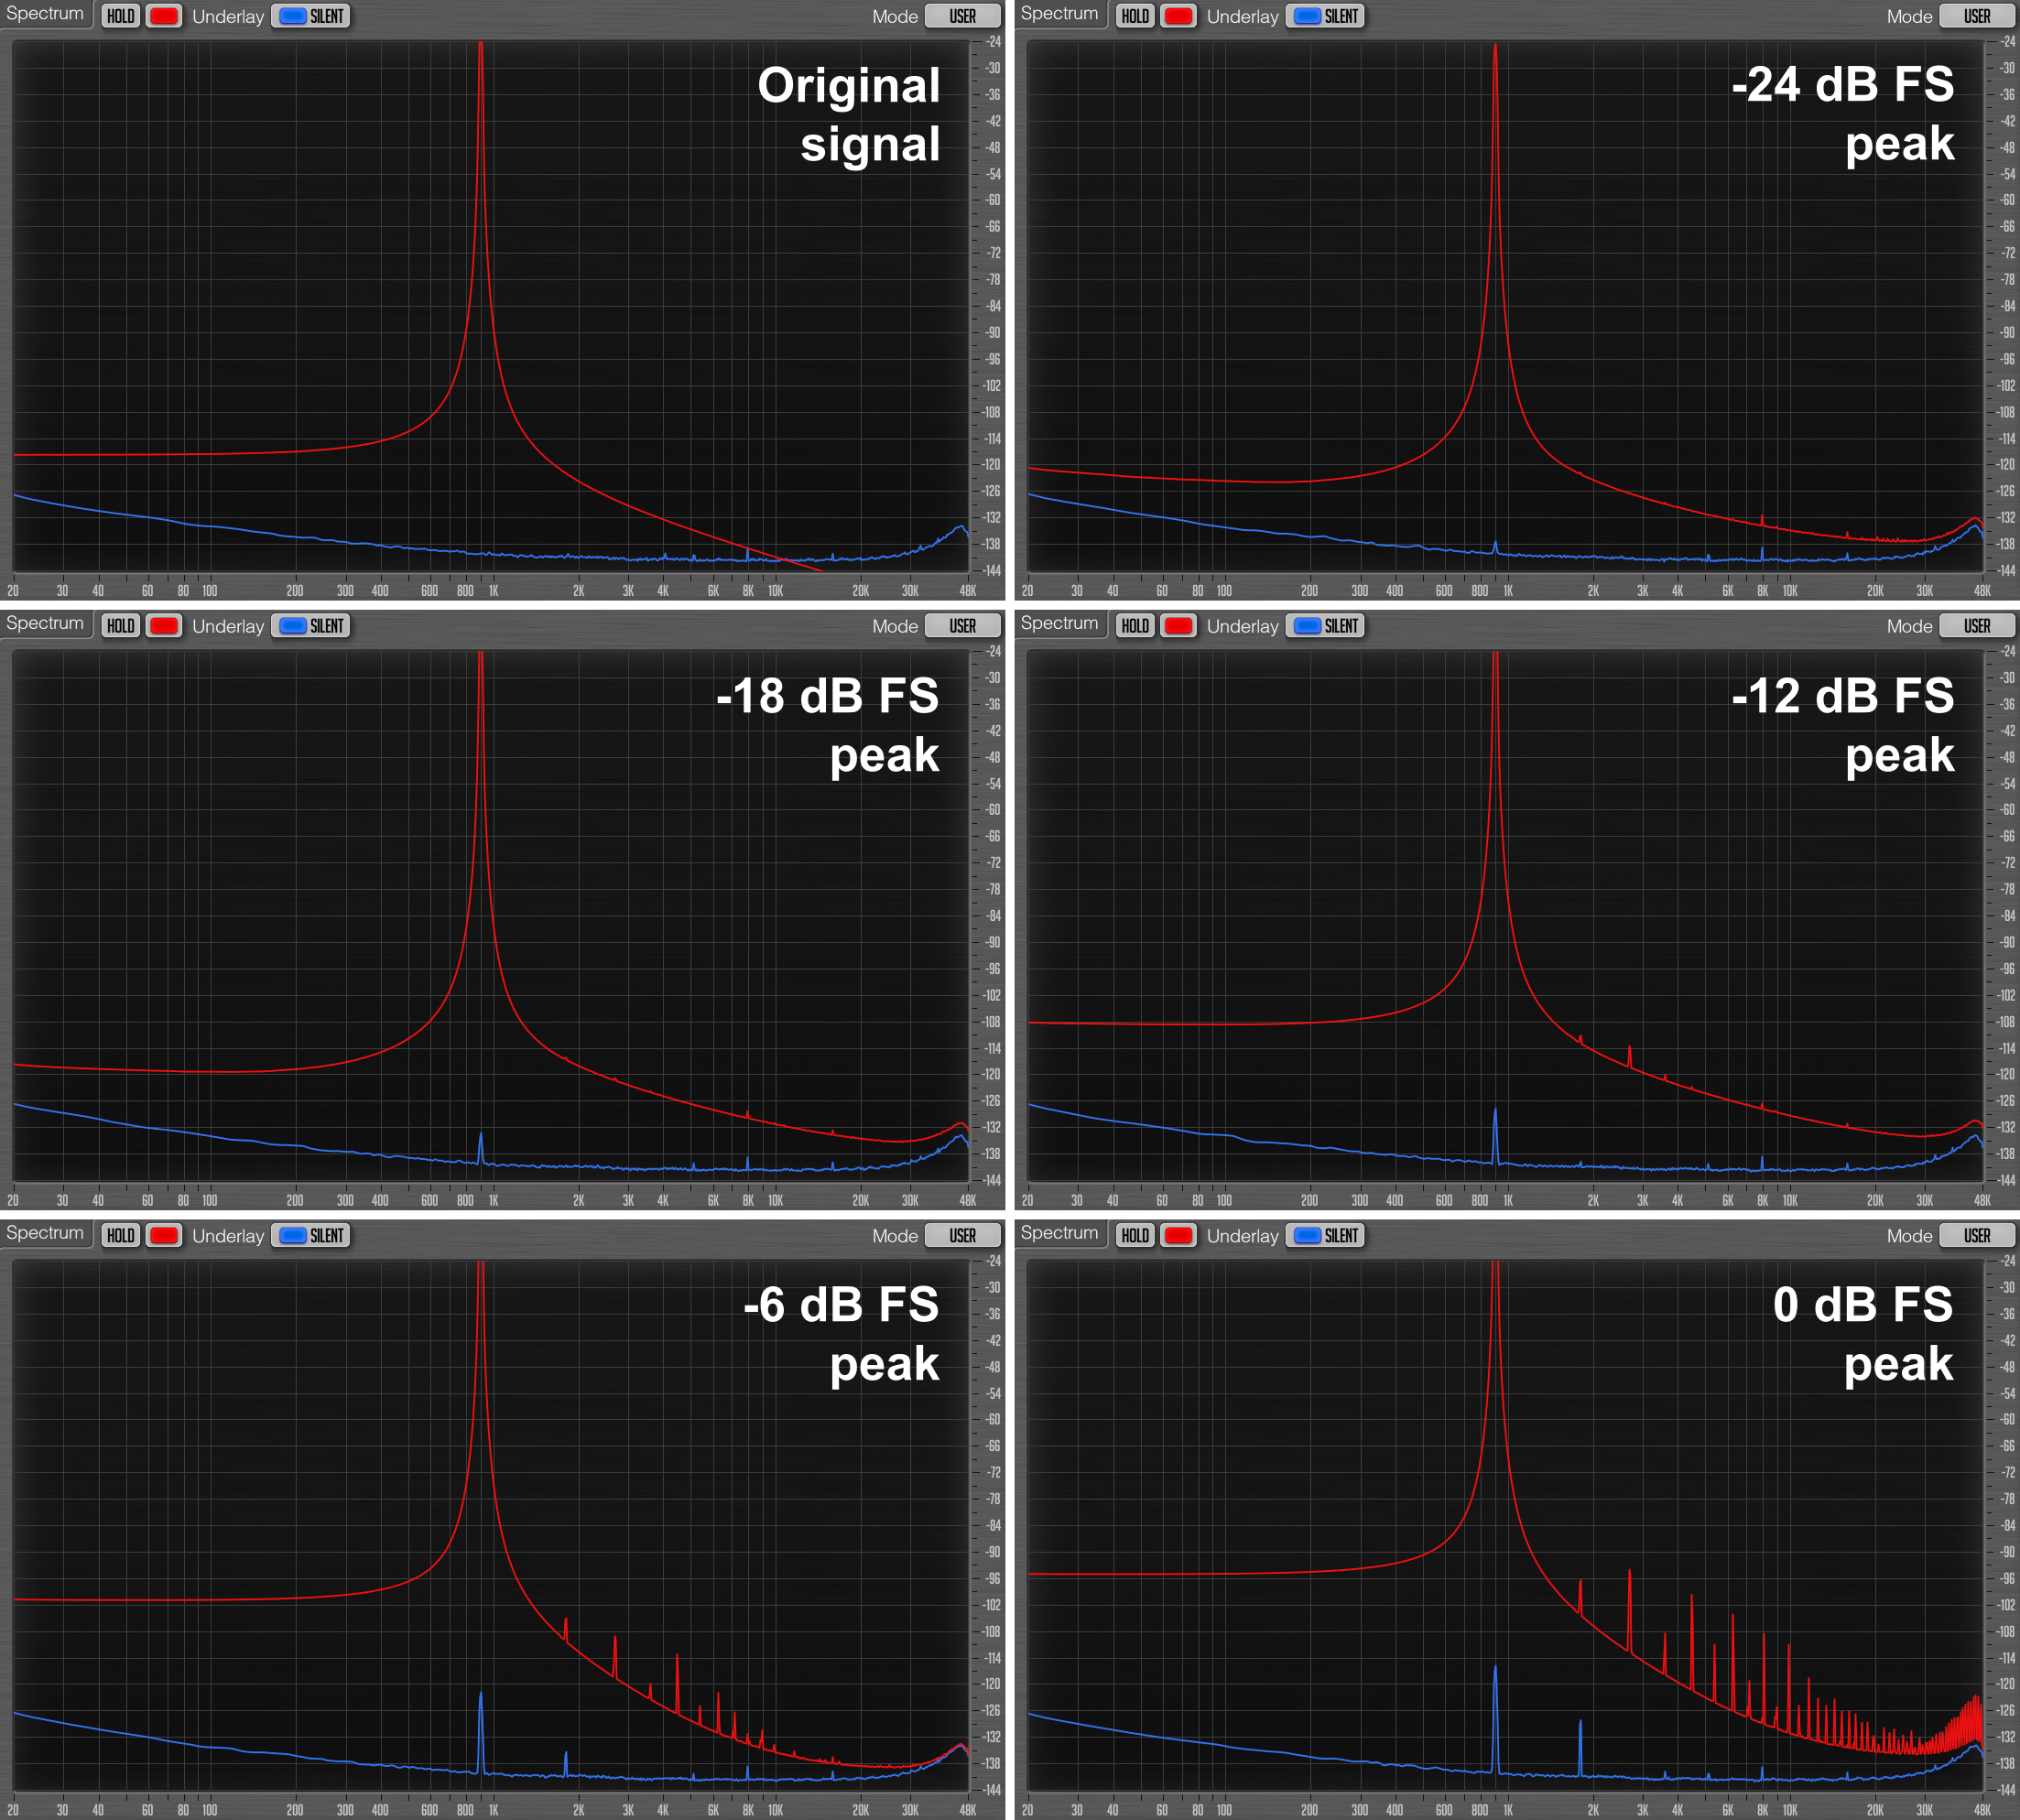
\includegraphics[scale=0.19,clip]{include/images/clipping_sine_ff800.png}

\subsection{Complex signal (several sine waves)}

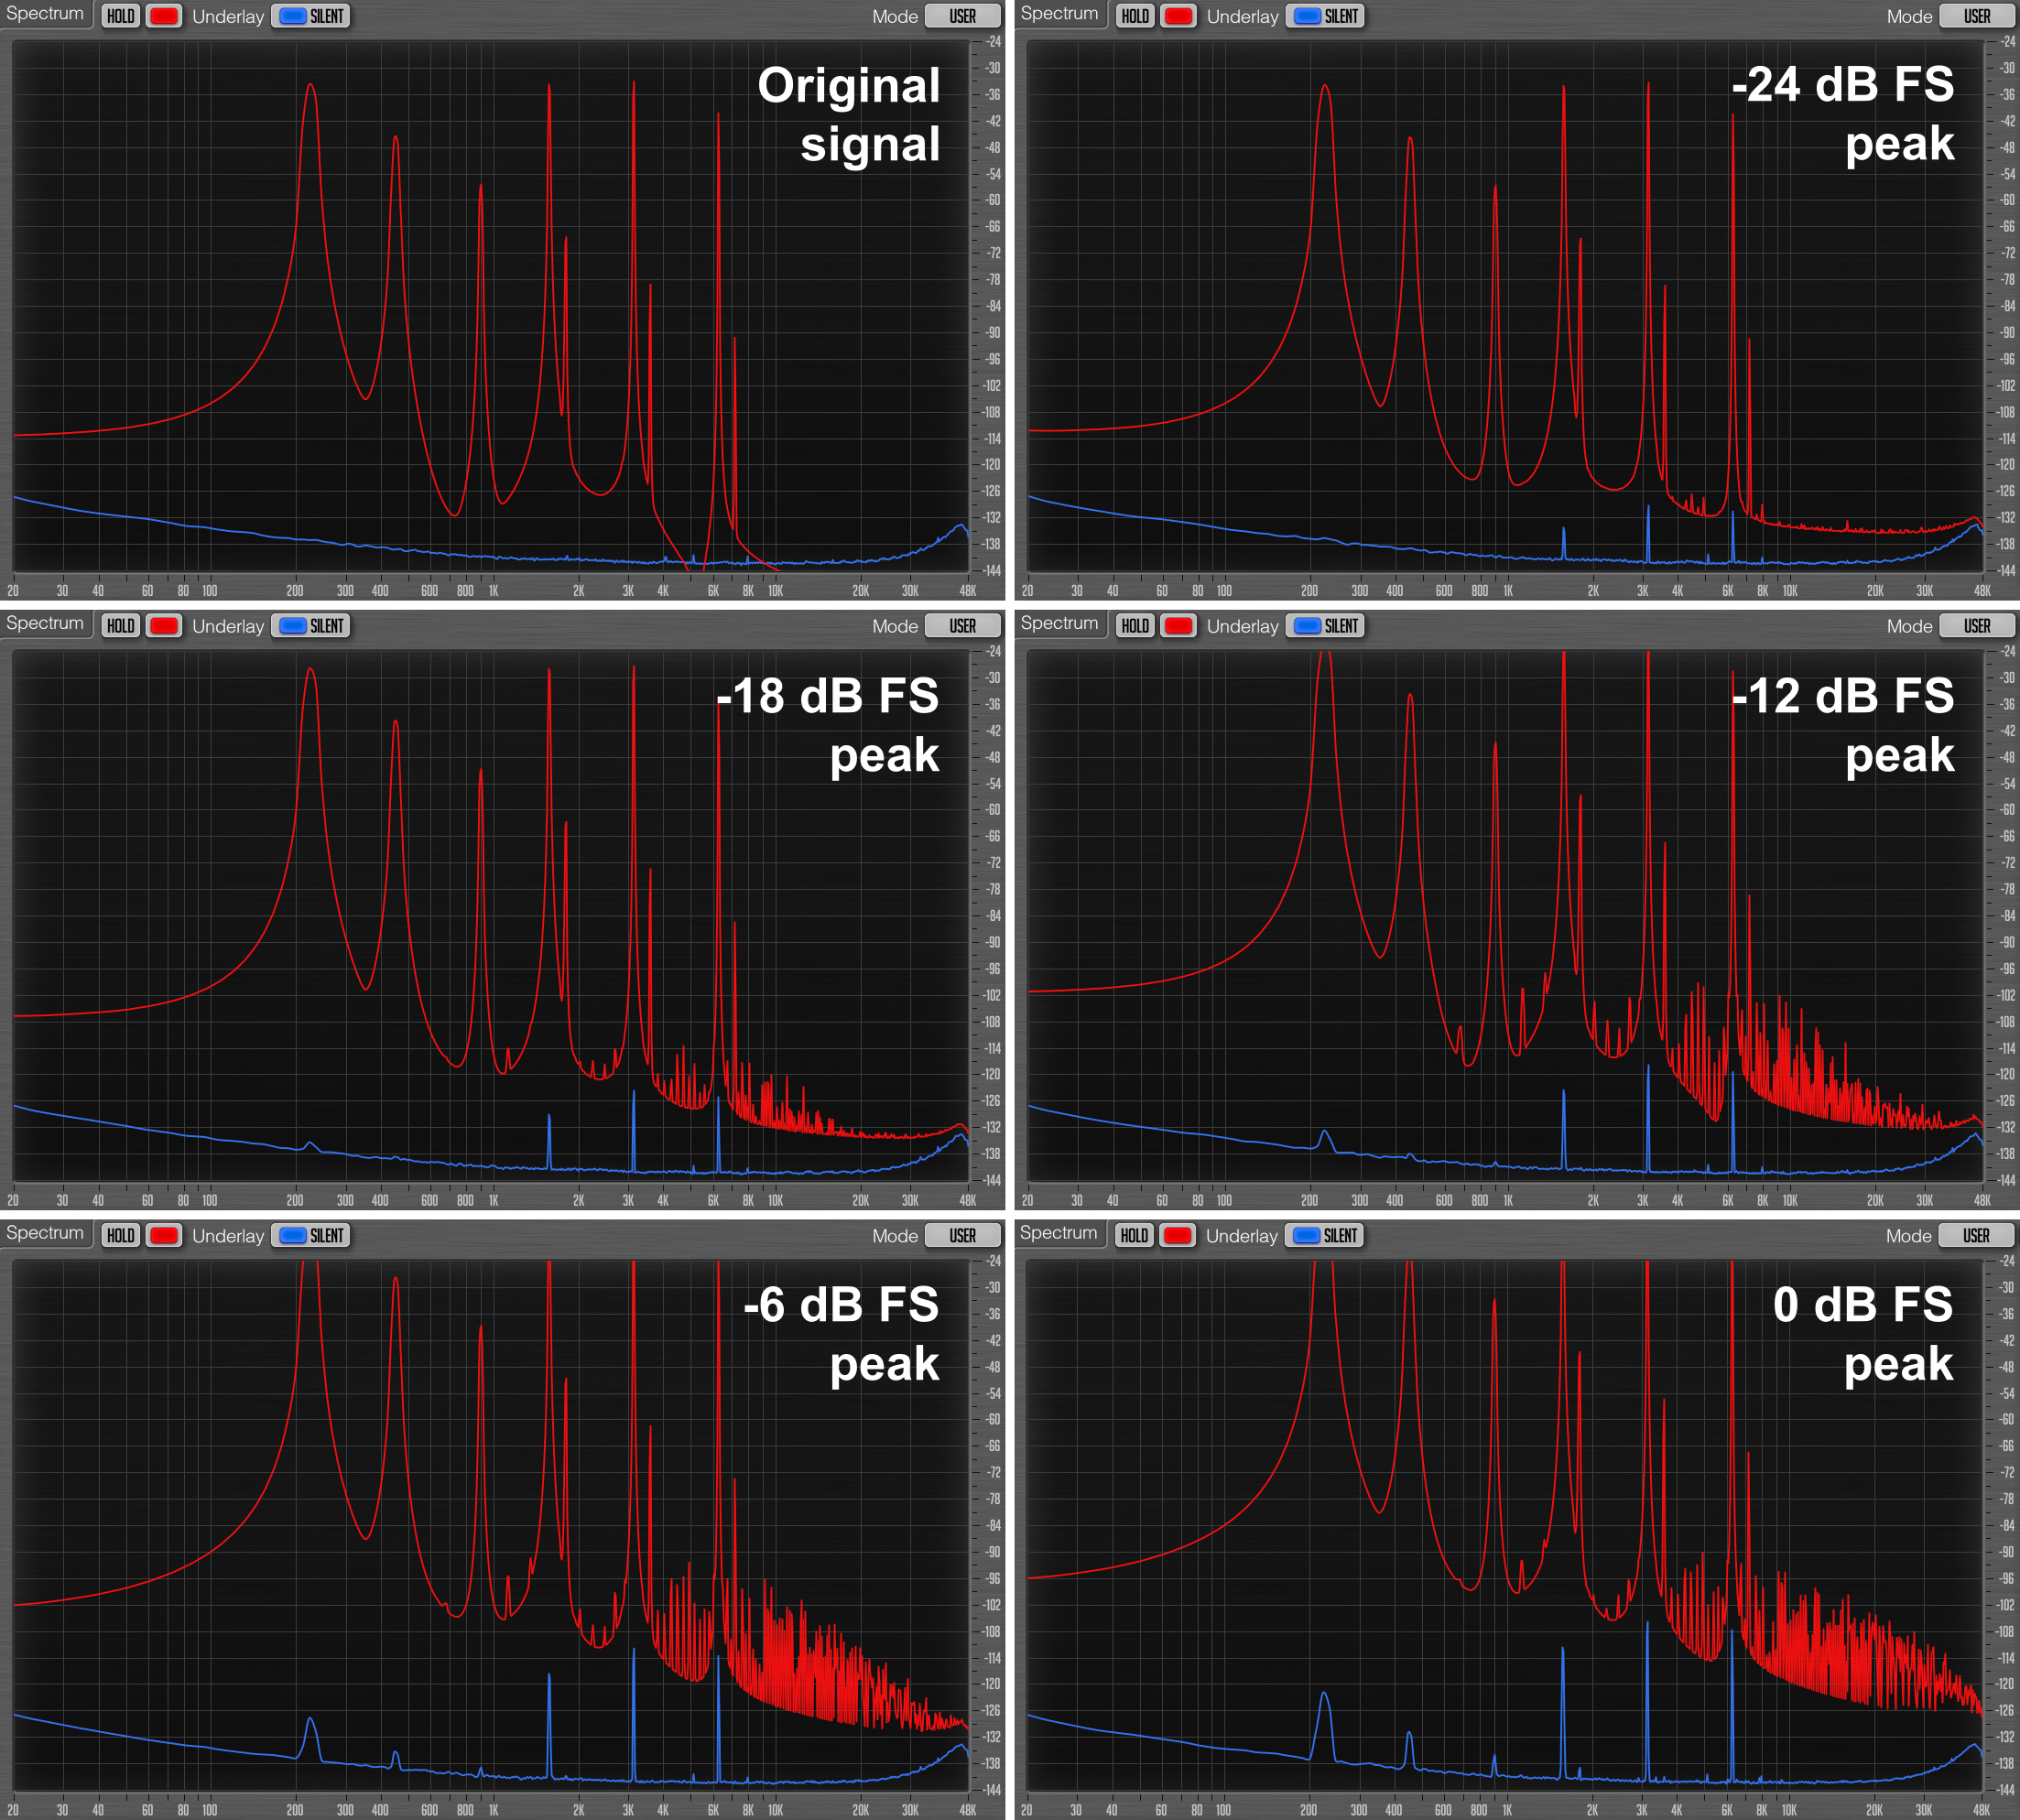
\includegraphics[scale=0.19,clip]{include/images/clipping_harmonics_ff800.png}

\chapter{traKmeter}
\label{chap:trakmeter}

\begin{wrapfigure}{r}{0.21\linewidth}
  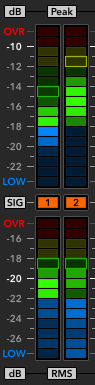
\includegraphics[scale=\screenshotscale,clip]{include/images/level_meter_complete.png}
\end{wrapfigure}

traKmeter consists of two meters, a peak meter on top and an average
meter below.  The meters are separated by an orange signal LED and
consist of a green area that is enclosed by a blue one (lower levels)
or a yellow and red one (higher levels).

The average meter's green area is centred around the
\textbf{\SI{-10}{\dBr} RMS} mark.  With a reference level of
\SI{-10}{\dBFS}, this corresponds to the \textbf{\SI{-20}{\dBFS} RMS}
we have determined to be the optimal average recording level in the
digital domain.

The peak meter's yellow area reaches up to \textbf{\SI{0}{\dBr} peak}.
Given the same reference level, this corresponds to
\textbf{\SI{-10}{\dBFS} peak} and peak levels shouldn't exceed this
level.

Thus, by keeping the meter's readout \textbf{in the green} and yellow
areas and \textbf{out of the red} areas, you will automatically track
at optimal audio levels.  It's as simple as that!

\section{Tracking with traKmeter}
\label{sec:tracking_with_trakmeter}

Open up an instance of traKmeter and set it up so that it measures
your audio input.  That can be done either by starting the stand-alone
version and connecting it to one or more input channels of your
analogue-to-digital converter, or by inserting a plug-in instance into
an input channel of your digital audio workstation (no latency is
added).

In the second case, take care that your digital audio workstation
doesn't add additional headroom and that no processing takes place
before traKmeter.  This can be ascertained by feeding calibration
tones into your converter or by directly comparing the readouts of
stand-alone and plug-in version.

\begin{wrapfigure}{r}{0.42\linewidth}
  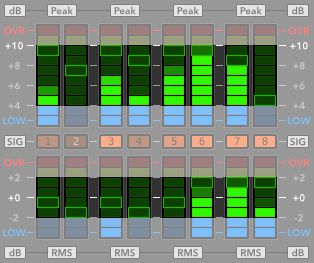
\includegraphics[scale=0.425,clip]{include/images/trakmeter_optimal.png}
\end{wrapfigure}

Now, feed the signal you want to record into an audio input channel
and adjust its level (in the analogue domain!).  Try to set the input
level so that it falls into the average meter's
\textbf{\SI{-10}{\dBr}} area.

Make sure that peak levels very rarely (if ever) exceed
\textbf{\SI{0}{\dBr}}.  In case both conditions cannot be met
simultaneously, adjust the peak level only.

\section{Mixing with traKmeter}
\label{sec:mixing_with_trakmeter}

When you get someone else's tracks for mixing, chances are that they
have been recorded far too hot.  While you can't change that, you
should adjust the tracks to optimal loudness in the gain staging
phase.  This is easily accomplished using traKmeter and either the
mixer's trim knob or a (properly dithered!) gain plug-in.  Just make
sure that the gain change precedes all future processing.

Mixing levels will now be much lower than what you might be used to.
This can easily be corrected by either adjusting the output gain of
your subgroups or by inserting a gain plug-in in your master track.

To preserve all transients, the final loudness of your mix should stay
within certain average level ranges.  My plug-in
\href{http://code.mzuther.de/}{\textbf{K-Meter}} may help you with
setting up correct mixing levels.  Remember that smashed transients
will be gone forever, whereas you can always bring up the volume
during mastering!

\chapter{Installation}
\label{chap:installation}

In order to use the pre-compiled binaries, simply extract the
traKmeter files from the downloaded archive.  For the plug-ins, you'll
then have to move the extracted files to your respective plug-in
folder.

\textbf{The folder} \path{trakmeter} \textbf{is mandatory and must be
  moved to the plug-in (or stand-alone) folder!}

traKmeter requires a processor which supports the SSE2 instruction
set.  On Windows, you might also have to install the
\href{https://www.visualstudio.com/downloads/}{Visual C++
  Redistributable for Visual Studio 2017}.

Should the stand-alone version ever fail to start, you can reset its
settings by deleting \path{traKmeter (Stereo).settings} or
\path{traKmeter (Multi).settings}.  These files are located in
\path{~/.config} (GNU/Linux) or \path{%appdata%\.config\} (Windows).

\chapter{Controls}
\label{chap:controls}

\section{Reference level buttons}
\label{sec:reference_level_buttons}

\begin{wrapfigure}{r}{0.14\linewidth}
  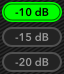
\includegraphics[scale=\screenshotscale,clip]{include/images/button_recording_level.png}
\end{wrapfigure}

Set your reference level (corresponding to the preferred maximum peak
recording level) with these buttons.  To follow the advice in
\ref{sec:gain_staging}, leave this at the default setting of
\textbf{\SI{-10}{\dBFS}}.

If you record very dynamic material or have problems getting a clean
signal, you can try the other settings.  They shift both meter scales
down by \SIrange{5}{10}{\dB} and add additional headroom at the cost
of a higher noise floor.  Which you probably won't even notice, as the
signal-to-noise ratio of modern converters is extremely high.

\section{Reset button}
\label{sec:reset_button}

\begin{wrapfigure}{r}{0.14\linewidth}
  
\includegraphics[scale=\screenshotscale,clip]{include/images/button_reset_on.png}
  \newline \vspace{-0.9\baselineskip}
  
\includegraphics[scale=\screenshotscale,clip]{include/images/button_reset_off.png}
\end{wrapfigure}

Click on this button to reset all meters.  This action will also
reload the current skin and re-draw everything.

\section{Select a skin}

\begin{wrapfigure}{r}{0.14\linewidth}
  
\includegraphics[scale=\screenshotscale,clip]{include/images/button_skin_on.png}
  \newline \vspace{-0.9\baselineskip}
  
\includegraphics[scale=\screenshotscale,clip]{include/images/button_skin_off.png}
\end{wrapfigure}

Click on this button to select the currently used traKmeter skin.  You
can also set a default skin that will be loaded when new plug-in
instances are started.

\section{Validation button}
\label{sec:validation_button}

\begin{wrapfigure}{r}{0.14\linewidth}
  
\includegraphics[scale=\screenshotscale,clip]{include/images/button_validate_on.png}
  \newline \vspace{-0.9\baselineskip}
  
\includegraphics[scale=\screenshotscale,clip]{include/images/button_validate_off.png}
\end{wrapfigure}

Click on this button to open the \textbf{validation window} (see
\ref{chap:validation}) which allows you to play an audio file through
traKmeter and dump internal data.  During validation, the button will
light up and clicking on it will stop validation early.

On Linux, dumped data will be written to \path{stderr}, so just start
the traKmeter stand-alone or your plug-in host from the shell and
watch the output coming.  On Windows, you can use DebugView by
Sysinternals (stand-alone) or have a look at Ableton Live's log files
(plug-in).  If none of that works, you might have to start either the
stand-alone or your plug-in host from a debugger.

As a side note, \textbf{SMA(50)} designates the simple moving average
of \num{50} values, a neat way to emphasise trends and eliminate
short-term fluctuations.

\section{About button}

\begin{wrapfigure}{r}{0.14\linewidth}
  
\includegraphics[scale=\screenshotscale,clip]{include/images/button_about_on.png}
  \newline \vspace{-0.9\baselineskip}
  
\includegraphics[scale=\screenshotscale,clip]{include/images/button_about_off.png}
\end{wrapfigure}

Clicking on this button will open the \textbf{about window} where you
will be informed about version number, contributors, copyright and the
GNU General Public License.

\section{Display license}

\begin{wrapfigure}{r}{0.15\linewidth}
  
\includegraphics[scale=\screenshotscale,clip]{include/images/button_gpl_on.png}
  \newline \vspace{-0.9\baselineskip}
  
\includegraphics[scale=\screenshotscale,clip]{include/images/button_gpl_off.png}
\end{wrapfigure}

This button is located in the \textbf{about window} and does not only
advertise that you are using free software licensed under the
\textbf{GNU General Public License} -- when clicked, it will also open
the license's website in your web browser \dots

\chapter{Meters}
\label{chap:meters}

All meters possess a flat frequency response.  Meter scales are in
\si{\dBr} and their reference level is adjustable (see
\ref{sec:reference_level_buttons}).  This way, scales remain the same
even when the reference level changes.

\section{Peak level meter}

\begin{wrapfigure}[6]{r}{0.21\linewidth} %% layout [number of narrow lines]
  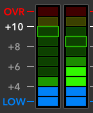
\includegraphics[scale=\screenshotscale,clip]{include/images/level_meter_peak.png}
\end{wrapfigure}

This meter shows the current peak level in \si{\dBr}.  Rise time is
one sample and fall time is \SI{8.67}{\dB\per\second}.  Peak levels
exceeding \SI{0}{\dBr} are displayed on the red LED marked ``OVR''.

The highest encountered peak level will be held indefinitely until the
meter is reset.

\newpage %% layout

\section{Average level meter}

\begin{wrapfigure}{r}{0.21\linewidth}
  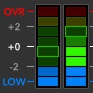
\includegraphics[scale=\screenshotscale,clip]{include/images/level_meter_average.png}
\end{wrapfigure}

The average level meter uses an averaging period of \num{1024}
samples.  It has been calibrated so that sine wave signals read the
same on both peak and average meters.  Similar to a VU meter, it takes
\SI{300}{\milli\second} for the meter to reach \SI{99}{\percent} of
the final reading.  There is no overshoot, however.

Peaks will be held for \SI{10}{\second} and then fall with a speed of
\SI{8.67}{\dB\per\second}.

\section{Signal meter}

\begin{wrapfigure}{r}{0.21\linewidth}
  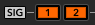
\includegraphics[scale=\screenshotscale,clip]{include/images/level_meter_signal.png}
\end{wrapfigure}

The orange signal meter detects peak levels at a threshold of
\SI{-60}{\dBFS}.  It has a rise time of one sample and fades out when
the level falls below the threshold.

\chapter{Recording advice}
\label{chap:recording_advice}

Over the years, I have learned how to and how not to record, and this
seems like a good place to summarise my knowledge.  For controversial
advice, I will try to reference the opinion of professionals.

\begin{description}

\item[Use a good pre-amplifier.]  ``Good'' doesn't mean your
  pre-amplifier has to have a lot of channels or features.  To the
  contrary!  Go for a simple design and invest your money in
  professional quality instead.  Recordings made with a good
  pre-amplifier sound better and make mixing much easier -- the tracks
  simply seem to fall into place.

\item[ Use the pre-amplifier's gain control.]  If necessary, crank up
  the gain control to yield the correct output level.  Do not fear the
  pre-amplifier's internal noise -- boosting a low-gain recording in
  later stages will result in even more noise!

\item[Avoid unbalanced equipment.]  Run all signals on balanced lines
  with a nominal level of \SI[retain-explicit-plus]{+4}{\dBu}.  If you
  can't, use DI boxes and transformers to convert the signals as early
  in the audio chain as possible.

  And do not even \emph{think} of buying equipment that has analogue
  RCA connectors!\footnote{``I have a real aversion to anything that
    calls itself `professional' and has RCA jacks on it.  That's just
    contradictory.'' \\
    \textbf{Whitlock B.}  \href{http://www.aes.org/live/?ID=218}{Audio
      System Grounding \& Interfacing -- An Overview.} \emph{126th AES
      Convention; Munich; May 2009.}}

\item[Use short audio chains.]  All equipment adds noise or may
  otherwise degrade audio, so keep your audio recording chains short
  and simple.  This has the additional benefit that you can focus on
  recording.

  Here is an example: instead of routing your mixer between
  pre-amplifier and converter, connect the mixer to your converter's
  outputs.  This simple change can lead to much better recordings
  (especially with cheap mixers) and the artist will still be able to
  hear playback and herself during recording.

\item[Work at a defined reference level.]  See the article
  \href{https://www.digido.com/portfolio-item/level-practices-part-1/}{Level
    Practices (Part 1)} by Bob Katz.

\item[Record at lower levels.]  During recording, do not let peak
  levels exceed \textbf{\SI{-10}{\dBFS}}.  For an in-depth explanation
  and references, see \ref{sec:gain_staging}.

\item[Record in mono.]  Most audio sources do not contain stereo
  information that is useful in a mixing context (notable exceptions
  are audience recordings, orchestras and occasionally pianos).  The
  pseudo-stereo effects of synthesizers often cause phasing issues.

  Recording such sources in stereo wastes space on your hard disk --
  and someone's time at a later stage.

\item[Use high bit depths.]  Do yourself a favour and record at a bit
  depth of \SI{24}{\bits} instead of \SI{16}{\bits}.  The additional
  bits allow recording at lower levels and provide an incredible
  amount of extra detail.  When disk space runs low, choose more bits
  over a higher sampling rate.\footnote{see the
    \href{http://www.aes.org/par/d/\#data_converter_bits}{AES Pro
      Audio Reference} for more information}

  The usable bit depth of converters is limited to approximately
  \SI{20}{\bits} by thermal noise.  However, the mixer in your digital
  audio workstation should use floating point numbers with
  \SI{32}{\bits} \emph{at the very least}.  Calculation errors are
  inevitable in digital signal processing, so more bits mean smaller
  (and thus quieter) errors.

\item[Use sensible sampling rates.]  The preferred sampling rate for
  recording audio is \SI{96}{\kilo\hertz} (\SI{88.1}{\kilo\hertz} is
  just as good, but sees less support).\footnote{``Although
    \SI{60}{\kilo\hertz} would [be ideal], \SI{88.2}{\kilo\hertz} and
    \SI{96}{\kilo\hertz} are closest to the optimal sample rate.''  I
    highly recommend
    reading this paper! \\
    \textbf{Lavry D.}
    \href{http://www.lavryengineering.com/lavry-white-papers/}{The
      Optimal Sample Rate For Quality Audio.} \emph{Lavry Engineering;
      White Paper; May 2012.}}  Additionally, latency is lower at
  higher sample rates, and many plug-ins that internally use
  \SI{96}{\kilo\hertz} can bypass their oversampling.

\item[Concentrate on recording.]  When tracking, try to not interfere
  with the flow of the session.  Keep editing and mixing to the bare
  minimum!

\item[Fix it now.]  Contrary to popular belief, you cannot ``fix it in
  the mix'' -- a bad recording is nothing more than a bad recording.
  So editing and tools like Auto-Tune and extreme EQ should be seen as
  a last resort.

  Apart from the precious time lost in editing, it's easy to kill all
  of a track's vibe in the process.

  Instead, keep recording until you capture a great take.  Treat your
  room acoustically and in terms of positive vibe.  Experiment with
  microphone placement.  And try absolutely everything that may help
  the artist in achieving a stunning performance!

\item[Make it exciting.]  A lot of today's music sounds like (and
  actually is) one short loop that was ``arranged'' by muting
  different tracks at different times.  This takes away all the small
  inaccuracies of human players and often leads to boring and lifeless
  songs.

  So think of a good arrangement before you even start recording.  And
  instead of looping a track, record a couple of takes and comp the
  best ones.  You'll be surprised at the difference it makes!

\end{description}

\chapter{Validation}
\label{chap:validation}

I have gone to great lengths to ensure that the meters read correctly.
You want to validate for yourself?  Just download and extract the
source code.  The directory \path{validation} contains instructions
and FLAC-compressed wave files.  A word of warning: these audio files
may \textbf{damage your ears} and speakers, so please watch your
monitor levels!

Begin by starting traKmeter.  If in a Bash shell, try this:

\begin{VerbatimBoth}
  ./trakmeter_stereo 2>&1 | tee /tmp/validate.log
\end{VerbatimBoth}

\begin{wrapfigure}{r}{0.32\linewidth}
  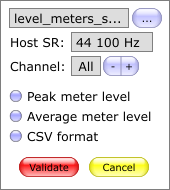
\includegraphics[scale=0.60,clip]{include/images/dialog_validation.png}
\end{wrapfigure}

After opening the \textbf{validation window} (see
\ref{sec:validation_button}), click on the ellipsis button (the one
with the dots) to select an audio file for playback through traKmeter.
Please make sure that the sampling rates of your host (\textbf{Host
  SR}) and the audio file match, otherwise the results will not be
correct.

Now, select which \textbf{variables} (if any) should be dumped.  You
may also restrict dumped data to a specific audio \textbf{channel}.
Check \textbf{CSV} if you want to feed the output to a parser.

Finally, click on the \textbf{validate} button to reset all meters and
start playback of the selected audio file.  All audio input will be
discarded during playback and for an additional twenty seconds.  To
stop playback early, simply click on the \textbf{validate} button
again.

\section{Validation status}

\begin{minipage}{1.0\linewidth}
  \renewcommand{\thempfootnote}{\arabic{mpfootnote}}
  \begin{tabular}{>{\bfseries}llcc}

    &
    \textbf{Test} &
    \textbf{Valid} \\

    Average level meter &
    visuals &
    \Checkmark{} \\

    &
    readout &
    \Checkmark{} \\

    Peak level meter &
    visuals &
    \Checkmark{} \\

    &
    readout &
    \Checkmark{} \\

    Signal meter &
    visuals &
    \Checkmark{} \\

  \end{tabular}
\end{minipage}

\chapter{Help needed}
\label{chap:help_needed}

As traKmeter was coded using cross-platform code, it should be easy to
compile on Mac OS X.  Unfortunately, I happen to not have a Mac \dots

In case you want to help, please see the next chapter for an email
address.  You’ll need sufficient experience in coding, compiling and
debugging, though, so no beginners please!

\chapter{Final words}
\label{chap:final_words}

I want to thank \textbf{Rickard} of Interfearing Sounds for asking me
how to use K-Meter for tracking.  This question and the following
thoughts really got traKmeter started.  I'd like to thank
\textbf{bram@smartelectronix} for his code to calculate logarithmic
rise and fall times.

I must also thank the \textbf{beta testers} and \textbf{users of
  traKmeter} for sending kind words, suggestions and bug reports.
Finally, I want to thank the \textbf{open source community} for making
all of this possible.

Although coding traKmeter has been a lot of fun, it has also been a
lot of work.  So if you like traKmeter, why not
\href{http://www.mzuther.de/}{send me an email} and tell me so?  Write
a few words about yourself, send suggestions for future updates or
volunteer to create a nice skin.  I also really enjoy listening to
music that you have produced using my software \dots

\emph{Thanks for using free software.  I hope you'll enjoy it!}

\appendix

\chapter{Build process}
\label{chap:build_process}

\section{Dependencies}
\label{sec:dependencies}

\subsection{premake}
\label{sec:dependencies_premake}

\begin{tabbing}
  \hspace*{6em}\=\=\kill

  Importance:  \> required \\
  Version:     \> 5.0.0 (alpha15) \\
  License:     \> BSD \\
  Homepage:    \> \href{https://premake.github.io/}{premake.github.io}
\end{tabbing}

\subsubsection{Installation}

Place the binary somewhere in your \path{PATH}.  Depending on your
platform, you should run \path{premake} using the scripts
\path{Builds/render_templates.sh} or
\path{Builds/render_templates.bat}.

To change the premake file using Jinja templates, you'll also have to
install the necessary dependencies.

\subsection{Compilers}

\begin{tabbing}
  \hspace*{6em}\=\=\kill

  Importance:  \> required \\
  Linux:       \> Clang 10.0 (or gcc 9.3.0) \\
  Windows:     \> Visual Studio 2019 (and above) \\
  License:     \> proprietary (Visual Studio) / Open Source \\
\end{tabbing}

Use premake (\ref{sec:dependencies_premake}) to generate the Make
files (or project) files needed by different compilers.

\emph{Different compiler versions may work, and premake supports other
  compiler tool sets as well.  But in this case, you're on your own!}

\subsection{JUCE library}

\begin{tabbing}
  \hspace*{6em}\=\=\kill

  Importance:  \> required \\
  Version:     \> 6.0.5 \\
  License:     \> ISC and GPL v3 (among others) \\
  Homepage:    \> \href{http://www.juce.com/}{www.juce.com}
\end{tabbing}

\subsubsection{Installation}

Extract the archive into the directory \path{libraries/juce}.

\subsection{Virtual Studio Technology SDK}

\begin{tabbing}
  \hspace*{6em}\=\=\kill

  Importance:  \> optional \\
  Version:     \> 2.4 / 3.6.14 \\
  License:     \> proprietary / GPL v3 \\
  Homepage:    \> \href{http://www.steinberg.net/en/company/developer.html}{www.steinberg.net}
\end{tabbing}

\subsubsection{Installation}

Extract the archives into the directories \path{libraries/vst2} and
\path{libraries/vst3}.  The proprietary VST2 SDK is not available
anymore.  \textbf{You may only distribute VST2 plug-ins if you have
  signed the old license agreement!}

\subsection{Python}

\begin{tabbing}
  \hspace*{6em}\=\=\kill

  Importance:  \> optional \\
  Version:     \> 3.8 (or higher) \\
  License:     \> Python Software Foundation License \\
  Homepage:    \> \href{http://www.python.org/}{www.python.org}
\end{tabbing}

You'll only need Python if you want to auto-generate files from Jinja
templates.

\subsubsection{Installation (Windows)}

You can download an installer from the website.

\subsection{Jinja}

\begin{tabbing}
  \hspace*{6em}\=\=\kill

  Importance:  \> optional \\
  Version:     \> 2.10 (or higher) \\
  License:     \> BSD \\
  Homepage:    \> \href{http://jinja.pocoo.org/}{jinja.pocoo.org}
\end{tabbing}

You'll only need Jinja if you want to auto-generate files such as the
premake file from templates (see \ref{sec:dependencies_premake}).

\subsection{Artistic Style}

\begin{tabbing}
  \hspace*{6em}\=\=\kill

  Importance:  \> optional \\
  Version:     \> 3.1 \\
  License:     \> LGPL v3 \\
  Homepage:    \> \href{http://astyle.sourceforge.net/}{astyle.sourceforge.net}
\end{tabbing}

This application formats the code so it looks more beautiful and
consistent.  Thus, you only have to install it if you plan to help me
with coding.

\subsubsection{Installation}

Place the binary somewhere in your \path{PATH}.  Depending on your
platform, you should run \path{astyle} using the scripts
\path{Source/format_code.sh} or \path{Source/format_code.bat}.

\subsection{googletest}

\begin{tabbing}
  \hspace*{6em}\=\=\kill

  Importance:  \> optional \\
  Version:     \> 1.10.0 \\
  License:     \> BSD 3-clauses \\
  Homepage:    \> \href{https://github.com/google/googletest}{github.com/google/googletest}
\end{tabbing}

This is a framework for testing and mocking.  You only need to install
it if you plan to help me with coding.

\subsubsection{Installation on GNU/Linux}

Extract the archive into the directory \path{libraries/googletest},
change into this directory and run:

\begin{VerbatimBoth}
  mkdir googletest/build
  cd googletest/build
\end{VerbatimBoth}

\begin{Verbatim64}
  rm -f ./CMakeCache.txt
  cmake ..
  make
  mkdir -p lib/linux/amd64/
  mv lib/*.a lib/linux/amd64/
  make clean
\end{Verbatim64}

\section{General preparation}
\label{sec:general_preparation}

Copy \path{Source/build_id-COPY.h} to \path{Source/build_id.h}.

Edit the copied file to add a custom build ID to the "About" dialog.
Or set up Git hooks that update the file for you.

\newpage %% layout

\section{GNU/Linux}

\subsection{Environment}

\emph{Supporting 32-bit Linux has become very tedious in the last
  years, so I have officially dropped it.  But it should be easy to
  adapt these instructions to 32-bit systems.}

To build this application yourself, I recommend setting up a
\texttt{chroot} environment.  This is fast and easy to do on
Debian-based systems and might save you a \textbf{lot} of trouble.  At
the time of writing, I'm using Linux Mint 20, but the procedure should
be similar on your distribution of choice.

Start by installing the necessary packages:

\begin{VerbatimBoth}
  sudo apt install debootstrap schroot
\end{VerbatimBoth}

Then install the \texttt{chroot} base system by executing the
following statements:

\begin{Verbatim64}
  sudo debootstrap --variant=buildd \
    --arch amd64 focal \
    /srv/chroot/focal_amd64 \
    http://archive.ubuntu.com/ubuntu
\end{Verbatim64}

Running \path{debootstrap} will take some time.  Meanwhile, add the
following lines to \path{/etc/schroot/schroot.conf} (make sure you
remove all preceding white space so that each line begins in the first
column):

\begin{Verbatim64}
  [focal-amd64]
  description=Ubuntu focal (amd64)
  directory=/srv/chroot/focal_amd64
  profile=default
  personality=linux
  type=directory
  users=username
\end{Verbatim64}

Please make the necessary changes to \texttt{username}.  If you
experience problems, you can try to change \texttt{focal} to a
release name such as \texttt{buster}.

When \path{debootstrap} is done, log in as superuser:

\begin{Verbatim64}
  sudo schroot -c focal-amd64
\end{Verbatim64}

First, install a few packages (\path{less}, \path{mc} and \path{vim}
are optional, but might come in handy):

\begin{VerbatimBoth}
  apt update
  apt -y install bash-completion less vim
\end{VerbatimBoth}

Then, use \path{vim} to change a line in \path{/etc/apt/sources.list}
(please ignore the line break, it should be a single line):

\begin{VerbatimBoth}
  deb http://archive.ubuntu.com/ubuntu focal
  main restricted universe
\end{VerbatimBoth}

Now install the remaining packages:

\begin{VerbatimBoth}
  apt update
  apt -y install clang cmake mc libasound2-dev \
    libjack-jackd2-dev libpthread-workqueue-dev \
    mesa-common-dev xorg-dev
  apt clean
\end{VerbatimBoth}

If you like \path{bash} completion, you might also want to open the
file \path{/etc/bash.bashrc} and unquote these lines:

\begin{VerbatimBoth}
  # enable bash completion in interactive shells
  if [...]
    [a couple of lines...]
  fi
\end{VerbatimBoth}

Finally, log out and log in as normal user:

\begin{Verbatim64}
  schroot -c focal-amd64
\end{Verbatim64}

In this \path{chroot} shell, install the dependencies
(\ref{sec:dependencies}).  Congratulations -- you are now ready to
build!

\newpage %% layout

\subsection{Build}

After preparing the dependencies, start your \texttt{chroot}
environment

\begin{Verbatim64}
  schroot -c focal-amd64
\end{Verbatim64}

change into the directory \path{Builds} and execute

\begin{VerbatimBoth}
  ./render_templates.sh
  make config=CFG TARGET
\end{VerbatimBoth}

where \application{CFG} is \application{debug\_x64}, or
\application{release\_x64}, and \application{TARGET} is the version
you want to compile, such as \application{linux\_standalone\_stereo}.

In case you run into problems, you can try to switch compilers by
opening the file \texttt{run\_premake.sh} and using the premake
options \texttt{--cc=clang} or \texttt{--cc=gcc}.

The compiled binaries will end up in the directory \path{bin}.

\newpage %% layout

\section{Microsoft Windows}

\subsection{Build}

After setting up the dependencies, open the directory \path{Builds}
and execute

\begin{VerbatimBoth}
  ./render_templates.bat
\end{VerbatimBoth}

Then change into the directory \path{Builds/windows/vs20xx}, open the
project file with the corresponding version of Visual Studio and build
the project.

The compiled binaries will end up in the directory \path{bin}.

%%% Local Variables:
%%% mode: latex
%%% mode: outline-minor
%%% TeX-command-default: "Rubber"
%%% TeX-master: "../trakmeter"
%%% TeX-PDF-mode: t
%%% ispell-local-dictionary: "british"
%%% End:


\chapter{Licenses}

\scriptsize
\section{GNU General Public License}
\label{sec:gpl-3}

\begin{verbatim}

                    GNU GENERAL PUBLIC LICENSE
                       Version 3, 29 June 2007

 Copyright (C) 2007 Free Software Foundation, Inc. <http://fsf.org/>
 Everyone is permitted to copy and distribute verbatim copies
 of this license document, but changing it is not allowed.

                            Preamble

  The GNU General Public License is a free, copyleft license for
software and other kinds of works.

  The licenses for most software and other practical works are designed
to take away your freedom to share and change the works.  By contrast,
the GNU General Public License is intended to guarantee your freedom to
share and change all versions of a program--to make sure it remains free
software for all its users.  We, the Free Software Foundation, use the
GNU General Public License for most of our software; it applies also to
any other work released this way by its authors.  You can apply it to
your programs, too.

  When we speak of free software, we are referring to freedom, not
price.  Our General Public Licenses are designed to make sure that you
have the freedom to distribute copies of free software (and charge for
them if you wish), that you receive source code or can get it if you
want it, that you can change the software or use pieces of it in new
free programs, and that you know you can do these things.

  To protect your rights, we need to prevent others from denying you
these rights or asking you to surrender the rights.  Therefore, you have
certain responsibilities if you distribute copies of the software, or if
you modify it: responsibilities to respect the freedom of others.

  For example, if you distribute copies of such a program, whether
gratis or for a fee, you must pass on to the recipients the same
freedoms that you received.  You must make sure that they, too, receive
or can get the source code.  And you must show them these terms so they
know their rights.

  Developers that use the GNU GPL protect your rights with two steps:
(1) assert copyright on the software, and (2) offer you this License
giving you legal permission to copy, distribute and/or modify it.

  For the developers' and authors' protection, the GPL clearly explains
that there is no warranty for this free software.  For both users' and
authors' sake, the GPL requires that modified versions be marked as
changed, so that their problems will not be attributed erroneously to
authors of previous versions.

  Some devices are designed to deny users access to install or run
modified versions of the software inside them, although the manufacturer
can do so.  This is fundamentally incompatible with the aim of
protecting users' freedom to change the software.  The systematic
pattern of such abuse occurs in the area of products for individuals to
use, which is precisely where it is most unacceptable.  Therefore, we
have designed this version of the GPL to prohibit the practice for those
products.  If such problems arise substantially in other domains, we
stand ready to extend this provision to those domains in future versions
of the GPL, as needed to protect the freedom of users.

  Finally, every program is threatened constantly by software patents.
States should not allow patents to restrict development and use of
software on general-purpose computers, but in those that do, we wish to
avoid the special danger that patents applied to a free program could
make it effectively proprietary.  To prevent this, the GPL assures that
patents cannot be used to render the program non-free.

  The precise terms and conditions for copying, distribution and
modification follow.

                       TERMS AND CONDITIONS

  0. Definitions.

  "This License" refers to version 3 of the GNU General Public License.

  "Copyright" also means copyright-like laws that apply to other kinds of
works, such as semiconductor masks.

  "The Program" refers to any copyrightable work licensed under this
License.  Each licensee is addressed as "you".  "Licensees" and
"recipients" may be individuals or organizations.

  To "modify" a work means to copy from or adapt all or part of the work
in a fashion requiring copyright permission, other than the making of an
exact copy.  The resulting work is called a "modified version" of the
earlier work or a work "based on" the earlier work.

  A "covered work" means either the unmodified Program or a work based
on the Program.

  To "propagate" a work means to do anything with it that, without
permission, would make you directly or secondarily liable for
infringement under applicable copyright law, except executing it on a
computer or modifying a private copy.  Propagation includes copying,
distribution (with or without modification), making available to the
public, and in some countries other activities as well.

  To "convey" a work means any kind of propagation that enables other
parties to make or receive copies.  Mere interaction with a user through
a computer network, with no transfer of a copy, is not conveying.

  An interactive user interface displays "Appropriate Legal Notices"
to the extent that it includes a convenient and prominently visible
feature that (1) displays an appropriate copyright notice, and (2)
tells the user that there is no warranty for the work (except to the
extent that warranties are provided), that licensees may convey the
work under this License, and how to view a copy of this License.  If
the interface presents a list of user commands or options, such as a
menu, a prominent item in the list meets this criterion.

  1. Source Code.

  The "source code" for a work means the preferred form of the work
for making modifications to it.  "Object code" means any non-source
form of a work.

  A "Standard Interface" means an interface that either is an official
standard defined by a recognized standards body, or, in the case of
interfaces specified for a particular programming language, one that
is widely used among developers working in that language.

  The "System Libraries" of an executable work include anything, other
than the work as a whole, that (a) is included in the normal form of
packaging a Major Component, but which is not part of that Major
Component, and (b) serves only to enable use of the work with that
Major Component, or to implement a Standard Interface for which an
implementation is available to the public in source code form.  A
"Major Component", in this context, means a major essential component
(kernel, window system, and so on) of the specific operating system
(if any) on which the executable work runs, or a compiler used to
produce the work, or an object code interpreter used to run it.

  The "Corresponding Source" for a work in object code form means all
the source code needed to generate, install, and (for an executable
work) run the object code and to modify the work, including scripts to
control those activities.  However, it does not include the work's
System Libraries, or general-purpose tools or generally available free
programs which are used unmodified in performing those activities but
which are not part of the work.  For example, Corresponding Source
includes interface definition files associated with source files for
the work, and the source code for shared libraries and dynamically
linked subprograms that the work is specifically designed to require,
such as by intimate data communication or control flow between those
subprograms and other parts of the work.

  The Corresponding Source need not include anything that users
can regenerate automatically from other parts of the Corresponding
Source.

  The Corresponding Source for a work in source code form is that
same work.

  2. Basic Permissions.

  All rights granted under this License are granted for the term of
copyright on the Program, and are irrevocable provided the stated
conditions are met.  This License explicitly affirms your unlimited
permission to run the unmodified Program.  The output from running a
covered work is covered by this License only if the output, given its
content, constitutes a covered work.  This License acknowledges your
rights of fair use or other equivalent, as provided by copyright law.

  You may make, run and propagate covered works that you do not
convey, without conditions so long as your license otherwise remains
in force.  You may convey covered works to others for the sole purpose
of having them make modifications exclusively for you, or provide you
with facilities for running those works, provided that you comply with
the terms of this License in conveying all material for which you do
not control copyright.  Those thus making or running the covered works
for you must do so exclusively on your behalf, under your direction
and control, on terms that prohibit them from making any copies of
your copyrighted material outside their relationship with you.

  Conveying under any other circumstances is permitted solely under
the conditions stated below.  Sublicensing is not allowed; section 10
makes it unnecessary.

  3. Protecting Users' Legal Rights From Anti-Circumvention Law.

  No covered work shall be deemed part of an effective technological
measure under any applicable law fulfilling obligations under article
11 of the WIPO copyright treaty adopted on 20 December 1996, or
similar laws prohibiting or restricting circumvention of such
measures.

  When you convey a covered work, you waive any legal power to forbid
circumvention of technological measures to the extent such circumvention
is effected by exercising rights under this License with respect to
the covered work, and you disclaim any intention to limit operation or
modification of the work as a means of enforcing, against the work's
users, your or third parties' legal rights to forbid circumvention of
technological measures.

  4. Conveying Verbatim Copies.

  You may convey verbatim copies of the Program's source code as you
receive it, in any medium, provided that you conspicuously and
appropriately publish on each copy an appropriate copyright notice;
keep intact all notices stating that this License and any
non-permissive terms added in accord with section 7 apply to the code;
keep intact all notices of the absence of any warranty; and give all
recipients a copy of this License along with the Program.

  You may charge any price or no price for each copy that you convey,
and you may offer support or warranty protection for a fee.

  5. Conveying Modified Source Versions.

  You may convey a work based on the Program, or the modifications to
produce it from the Program, in the form of source code under the
terms of section 4, provided that you also meet all of these conditions:

    a) The work must carry prominent notices stating that you modified
    it, and giving a relevant date.

    b) The work must carry prominent notices stating that it is
    released under this License and any conditions added under section
    7.  This requirement modifies the requirement in section 4 to
    "keep intact all notices".

    c) You must license the entire work, as a whole, under this
    License to anyone who comes into possession of a copy.  This
    License will therefore apply, along with any applicable section 7
    additional terms, to the whole of the work, and all its parts,
    regardless of how they are packaged.  This License gives no
    permission to license the work in any other way, but it does not
    invalidate such permission if you have separately received it.

    d) If the work has interactive user interfaces, each must display
    Appropriate Legal Notices; however, if the Program has interactive
    interfaces that do not display Appropriate Legal Notices, your
    work need not make them do so.

  A compilation of a covered work with other separate and independent
works, which are not by their nature extensions of the covered work,
and which are not combined with it such as to form a larger program,
in or on a volume of a storage or distribution medium, is called an
"aggregate" if the compilation and its resulting copyright are not
used to limit the access or legal rights of the compilation's users
beyond what the individual works permit.  Inclusion of a covered work
in an aggregate does not cause this License to apply to the other
parts of the aggregate.

  6. Conveying Non-Source Forms.

  You may convey a covered work in object code form under the terms
of sections 4 and 5, provided that you also convey the
machine-readable Corresponding Source under the terms of this License,
in one of these ways:

    a) Convey the object code in, or embodied in, a physical product
    (including a physical distribution medium), accompanied by the
    Corresponding Source fixed on a durable physical medium
    customarily used for software interchange.

    b) Convey the object code in, or embodied in, a physical product
    (including a physical distribution medium), accompanied by a
    written offer, valid for at least three years and valid for as
    long as you offer spare parts or customer support for that product
    model, to give anyone who possesses the object code either (1) a
    copy of the Corresponding Source for all the software in the
    product that is covered by this License, on a durable physical
    medium customarily used for software interchange, for a price no
    more than your reasonable cost of physically performing this
    conveying of source, or (2) access to copy the
    Corresponding Source from a network server at no charge.

    c) Convey individual copies of the object code with a copy of the
    written offer to provide the Corresponding Source.  This
    alternative is allowed only occasionally and noncommercially, and
    only if you received the object code with such an offer, in accord
    with subsection 6b.

    d) Convey the object code by offering access from a designated
    place (gratis or for a charge), and offer equivalent access to the
    Corresponding Source in the same way through the same place at no
    further charge.  You need not require recipients to copy the
    Corresponding Source along with the object code.  If the place to
    copy the object code is a network server, the Corresponding Source
    may be on a different server (operated by you or a third party)
    that supports equivalent copying facilities, provided you maintain
    clear directions next to the object code saying where to find the
    Corresponding Source.  Regardless of what server hosts the
    Corresponding Source, you remain obligated to ensure that it is
    available for as long as needed to satisfy these requirements.

    e) Convey the object code using peer-to-peer transmission, provided
    you inform other peers where the object code and Corresponding
    Source of the work are being offered to the general public at no
    charge under subsection 6d.

  A separable portion of the object code, whose source code is excluded
from the Corresponding Source as a System Library, need not be
included in conveying the object code work.

  A "User Product" is either (1) a "consumer product", which means any
tangible personal property which is normally used for personal, family,
or household purposes, or (2) anything designed or sold for incorporation
into a dwelling.  In determining whether a product is a consumer product,
doubtful cases shall be resolved in favor of coverage.  For a particular
product received by a particular user, "normally used" refers to a
typical or common use of that class of product, regardless of the status
of the particular user or of the way in which the particular user
actually uses, or expects or is expected to use, the product.  A product
is a consumer product regardless of whether the product has substantial
commercial, industrial or non-consumer uses, unless such uses represent
the only significant mode of use of the product.

  "Installation Information" for a User Product means any methods,
procedures, authorization keys, or other information required to install
and execute modified versions of a covered work in that User Product from
a modified version of its Corresponding Source.  The information must
suffice to ensure that the continued functioning of the modified object
code is in no case prevented or interfered with solely because
modification has been made.

  If you convey an object code work under this section in, or with, or
specifically for use in, a User Product, and the conveying occurs as
part of a transaction in which the right of possession and use of the
User Product is transferred to the recipient in perpetuity or for a
fixed term (regardless of how the transaction is characterized), the
Corresponding Source conveyed under this section must be accompanied
by the Installation Information.  But this requirement does not apply
if neither you nor any third party retains the ability to install
modified object code on the User Product (for example, the work has
been installed in ROM).

  The requirement to provide Installation Information does not include a
requirement to continue to provide support service, warranty, or updates
for a work that has been modified or installed by the recipient, or for
the User Product in which it has been modified or installed.  Access to a
network may be denied when the modification itself materially and
adversely affects the operation of the network or violates the rules and
protocols for communication across the network.

  Corresponding Source conveyed, and Installation Information provided,
in accord with this section must be in a format that is publicly
documented (and with an implementation available to the public in
source code form), and must require no special password or key for
unpacking, reading or copying.

  7. Additional Terms.

  "Additional permissions" are terms that supplement the terms of this
License by making exceptions from one or more of its conditions.
Additional permissions that are applicable to the entire Program shall
be treated as though they were included in this License, to the extent
that they are valid under applicable law.  If additional permissions
apply only to part of the Program, that part may be used separately
under those permissions, but the entire Program remains governed by
this License without regard to the additional permissions.

  When you convey a copy of a covered work, you may at your option
remove any additional permissions from that copy, or from any part of
it.  (Additional permissions may be written to require their own
removal in certain cases when you modify the work.)  You may place
additional permissions on material, added by you to a covered work,
for which you have or can give appropriate copyright permission.

  Notwithstanding any other provision of this License, for material you
add to a covered work, you may (if authorized by the copyright holders of
that material) supplement the terms of this License with terms:

    a) Disclaiming warranty or limiting liability differently from the
    terms of sections 15 and 16 of this License; or

    b) Requiring preservation of specified reasonable legal notices or
    author attributions in that material or in the Appropriate Legal
    Notices displayed by works containing it; or

    c) Prohibiting misrepresentation of the origin of that material, or
    requiring that modified versions of such material be marked in
    reasonable ways as different from the original version; or

    d) Limiting the use for publicity purposes of names of licensors or
    authors of the material; or

    e) Declining to grant rights under trademark law for use of some
    trade names, trademarks, or service marks; or

    f) Requiring indemnification of licensors and authors of that
    material by anyone who conveys the material (or modified versions of
    it) with contractual assumptions of liability to the recipient, for
    any liability that these contractual assumptions directly impose on
    those licensors and authors.

  All other non-permissive additional terms are considered "further
restrictions" within the meaning of section 10.  If the Program as you
received it, or any part of it, contains a notice stating that it is
governed by this License along with a term that is a further
restriction, you may remove that term.  If a license document contains
a further restriction but permits relicensing or conveying under this
License, you may add to a covered work material governed by the terms
of that license document, provided that the further restriction does
not survive such relicensing or conveying.

  If you add terms to a covered work in accord with this section, you
must place, in the relevant source files, a statement of the
additional terms that apply to those files, or a notice indicating
where to find the applicable terms.

  Additional terms, permissive or non-permissive, may be stated in the
form of a separately written license, or stated as exceptions;
the above requirements apply either way.

  8. Termination.

  You may not propagate or modify a covered work except as expressly
provided under this License.  Any attempt otherwise to propagate or
modify it is void, and will automatically terminate your rights under
this License (including any patent licenses granted under the third
paragraph of section 11).

  However, if you cease all violation of this License, then your
license from a particular copyright holder is reinstated (a)
provisionally, unless and until the copyright holder explicitly and
finally terminates your license, and (b) permanently, if the copyright
holder fails to notify you of the violation by some reasonable means
prior to 60 days after the cessation.

  Moreover, your license from a particular copyright holder is
reinstated permanently if the copyright holder notifies you of the
violation by some reasonable means, this is the first time you have
received notice of violation of this License (for any work) from that
copyright holder, and you cure the violation prior to 30 days after
your receipt of the notice.

  Termination of your rights under this section does not terminate the
licenses of parties who have received copies or rights from you under
this License.  If your rights have been terminated and not permanently
reinstated, you do not qualify to receive new licenses for the same
material under section 10.

  9. Acceptance Not Required for Having Copies.

  You are not required to accept this License in order to receive or
run a copy of the Program.  Ancillary propagation of a covered work
occurring solely as a consequence of using peer-to-peer transmission
to receive a copy likewise does not require acceptance.  However,
nothing other than this License grants you permission to propagate or
modify any covered work.  These actions infringe copyright if you do
not accept this License.  Therefore, by modifying or propagating a
covered work, you indicate your acceptance of this License to do so.

  10. Automatic Licensing of Downstream Recipients.

  Each time you convey a covered work, the recipient automatically
receives a license from the original licensors, to run, modify and
propagate that work, subject to this License.  You are not responsible
for enforcing compliance by third parties with this License.

  An "entity transaction" is a transaction transferring control of an
organization, or substantially all assets of one, or subdividing an
organization, or merging organizations.  If propagation of a covered
work results from an entity transaction, each party to that
transaction who receives a copy of the work also receives whatever
licenses to the work the party's predecessor in interest had or could
give under the previous paragraph, plus a right to possession of the
Corresponding Source of the work from the predecessor in interest, if
the predecessor has it or can get it with reasonable efforts.

  You may not impose any further restrictions on the exercise of the
rights granted or affirmed under this License.  For example, you may
not impose a license fee, royalty, or other charge for exercise of
rights granted under this License, and you may not initiate litigation
(including a cross-claim or counterclaim in a lawsuit) alleging that
any patent claim is infringed by making, using, selling, offering for
sale, or importing the Program or any portion of it.

  11. Patents.

  A "contributor" is a copyright holder who authorizes use under this
License of the Program or a work on which the Program is based.  The
work thus licensed is called the contributor's "contributor version".

  A contributor's "essential patent claims" are all patent claims
owned or controlled by the contributor, whether already acquired or
hereafter acquired, that would be infringed by some manner, permitted
by this License, of making, using, or selling its contributor version,
but do not include claims that would be infringed only as a
consequence of further modification of the contributor version.  For
purposes of this definition, "control" includes the right to grant
patent sublicenses in a manner consistent with the requirements of
this License.

  Each contributor grants you a non-exclusive, worldwide, royalty-free
patent license under the contributor's essential patent claims, to
make, use, sell, offer for sale, import and otherwise run, modify and
propagate the contents of its contributor version.

  In the following three paragraphs, a "patent license" is any express
agreement or commitment, however denominated, not to enforce a patent
(such as an express permission to practice a patent or covenant not to
sue for patent infringement).  To "grant" such a patent license to a
party means to make such an agreement or commitment not to enforce a
patent against the party.

  If you convey a covered work, knowingly relying on a patent license,
and the Corresponding Source of the work is not available for anyone
to copy, free of charge and under the terms of this License, through a
publicly available network server or other readily accessible means,
then you must either (1) cause the Corresponding Source to be so
available, or (2) arrange to deprive yourself of the benefit of the
patent license for this particular work, or (3) arrange, in a manner
consistent with the requirements of this License, to extend the patent
license to downstream recipients.  "Knowingly relying" means you have
actual knowledge that, but for the patent license, your conveying the
covered work in a country, or your recipient's use of the covered work
in a country, would infringe one or more identifiable patents in that
country that you have reason to believe are valid.

  If, pursuant to or in connection with a single transaction or
arrangement, you convey, or propagate by procuring conveyance of, a
covered work, and grant a patent license to some of the parties
receiving the covered work authorizing them to use, propagate, modify
or convey a specific copy of the covered work, then the patent license
you grant is automatically extended to all recipients of the covered
work and works based on it.

  A patent license is "discriminatory" if it does not include within
the scope of its coverage, prohibits the exercise of, or is
conditioned on the non-exercise of one or more of the rights that are
specifically granted under this License.  You may not convey a covered
work if you are a party to an arrangement with a third party that is
in the business of distributing software, under which you make payment
to the third party based on the extent of your activity of conveying
the work, and under which the third party grants, to any of the
parties who would receive the covered work from you, a discriminatory
patent license (a) in connection with copies of the covered work
conveyed by you (or copies made from those copies), or (b) primarily
for and in connection with specific products or compilations that
contain the covered work, unless you entered into that arrangement,
or that patent license was granted, prior to 28 March 2007.

  Nothing in this License shall be construed as excluding or limiting
any implied license or other defenses to infringement that may
otherwise be available to you under applicable patent law.

  12. No Surrender of Others' Freedom.

  If conditions are imposed on you (whether by court order, agreement or
otherwise) that contradict the conditions of this License, they do not
excuse you from the conditions of this License.  If you cannot convey a
covered work so as to satisfy simultaneously your obligations under this
License and any other pertinent obligations, then as a consequence you may
not convey it at all.  For example, if you agree to terms that obligate you
to collect a royalty for further conveying from those to whom you convey
the Program, the only way you could satisfy both those terms and this
License would be to refrain entirely from conveying the Program.

  13. Use with the GNU Affero General Public License.

  Notwithstanding any other provision of this License, you have
permission to link or combine any covered work with a work licensed
under version 3 of the GNU Affero General Public License into a single
combined work, and to convey the resulting work.  The terms of this
License will continue to apply to the part which is the covered work,
but the special requirements of the GNU Affero General Public License,
section 13, concerning interaction through a network will apply to the
combination as such.

  14. Revised Versions of this License.

  The Free Software Foundation may publish revised and/or new versions of
the GNU General Public License from time to time.  Such new versions will
be similar in spirit to the present version, but may differ in detail to
address new problems or concerns.

  Each version is given a distinguishing version number.  If the
Program specifies that a certain numbered version of the GNU General
Public License "or any later version" applies to it, you have the
option of following the terms and conditions either of that numbered
version or of any later version published by the Free Software
Foundation.  If the Program does not specify a version number of the
GNU General Public License, you may choose any version ever published
by the Free Software Foundation.

  If the Program specifies that a proxy can decide which future
versions of the GNU General Public License can be used, that proxy's
public statement of acceptance of a version permanently authorizes you
to choose that version for the Program.

  Later license versions may give you additional or different
permissions.  However, no additional obligations are imposed on any
author or copyright holder as a result of your choosing to follow a
later version.

  15. Disclaimer of Warranty.

  THERE IS NO WARRANTY FOR THE PROGRAM, TO THE EXTENT PERMITTED BY
APPLICABLE LAW.  EXCEPT WHEN OTHERWISE STATED IN WRITING THE COPYRIGHT
HOLDERS AND/OR OTHER PARTIES PROVIDE THE PROGRAM "AS IS" WITHOUT WARRANTY
OF ANY KIND, EITHER EXPRESSED OR IMPLIED, INCLUDING, BUT NOT LIMITED TO,
THE IMPLIED WARRANTIES OF MERCHANTABILITY AND FITNESS FOR A PARTICULAR
PURPOSE.  THE ENTIRE RISK AS TO THE QUALITY AND PERFORMANCE OF THE PROGRAM
IS WITH YOU.  SHOULD THE PROGRAM PROVE DEFECTIVE, YOU ASSUME THE COST OF
ALL NECESSARY SERVICING, REPAIR OR CORRECTION.

  16. Limitation of Liability.

  IN NO EVENT UNLESS REQUIRED BY APPLICABLE LAW OR AGREED TO IN WRITING
WILL ANY COPYRIGHT HOLDER, OR ANY OTHER PARTY WHO MODIFIES AND/OR CONVEYS
THE PROGRAM AS PERMITTED ABOVE, BE LIABLE TO YOU FOR DAMAGES, INCLUDING ANY
GENERAL, SPECIAL, INCIDENTAL OR CONSEQUENTIAL DAMAGES ARISING OUT OF THE
USE OR INABILITY TO USE THE PROGRAM (INCLUDING BUT NOT LIMITED TO LOSS OF
DATA OR DATA BEING RENDERED INACCURATE OR LOSSES SUSTAINED BY YOU OR THIRD
PARTIES OR A FAILURE OF THE PROGRAM TO OPERATE WITH ANY OTHER PROGRAMS),
EVEN IF SUCH HOLDER OR OTHER PARTY HAS BEEN ADVISED OF THE POSSIBILITY OF
SUCH DAMAGES.

  17. Interpretation of Sections 15 and 16.

  If the disclaimer of warranty and limitation of liability provided
above cannot be given local legal effect according to their terms,
reviewing courts shall apply local law that most closely approximates
an absolute waiver of all civil liability in connection with the
Program, unless a warranty or assumption of liability accompanies a
copy of the Program in return for a fee.

                     END OF TERMS AND CONDITIONS

            How to Apply These Terms to Your New Programs

  If you develop a new program, and you want it to be of the greatest
possible use to the public, the best way to achieve this is to make it
free software which everyone can redistribute and change under these terms.

  To do so, attach the following notices to the program.  It is safest
to attach them to the start of each source file to most effectively
state the exclusion of warranty; and each file should have at least
the "copyright" line and a pointer to where the full notice is found.

    <one line to give the program's name and a brief idea of what it does.>
    Copyright (C) <year>  <name of author>

    This program is free software: you can redistribute it and/or modify
    it under the terms of the GNU General Public License as published by
    the Free Software Foundation, either version 3 of the License, or
    (at your option) any later version.

    This program is distributed in the hope that it will be useful,
    but WITHOUT ANY WARRANTY; without even the implied warranty of
    MERCHANTABILITY or FITNESS FOR A PARTICULAR PURPOSE.  See the
    GNU General Public License for more details.

    You should have received a copy of the GNU General Public License
    along with this program.  If not, see <http://www.gnu.org/licenses/>.

Also add information on how to contact you by electronic and paper mail.

  If the program does terminal interaction, make it output a short
notice like this when it starts in an interactive mode:

    <program>  Copyright (C) <year>  <name of author>
    This program comes with ABSOLUTELY NO WARRANTY; for details type `show w'.
    This is free software, and you are welcome to redistribute it
    under certain conditions; type `show c' for details.

The hypothetical commands `show w' and `show c' should show the appropriate
parts of the General Public License.  Of course, your program's commands
might be different; for a GUI interface, you would use an "about box".

  You should also get your employer (if you work as a programmer) or school,
if any, to sign a "copyright disclaimer" for the program, if necessary.
For more information on this, and how to apply and follow the GNU GPL, see
<http://www.gnu.org/licenses/>.

  The GNU General Public License does not permit incorporating your program
into proprietary programs.  If your program is a subroutine library, you
may consider it more useful to permit linking proprietary applications with
the library.  If this is what you want to do, use the GNU Lesser General
Public License instead of this License.  But first, please read
<http://www.gnu.org/philosophy/why-not-lgpl.html>.

\end{verbatim}

\normalsize

\scriptsize
\section{Creative Commons Attribution-ShareAlike 4.0 International}
\label{sec:cc-by-sa-4.0}

\begin{Verbatim}

Creative Commons Corporation ("Creative Commons") is not a law firm and
does not provide legal services or legal advice. Distribution of
Creative Commons public licenses does not create a lawyer-client or
other relationship. Creative Commons makes its licenses and related
information available on an "as-is" basis. Creative Commons gives no
warranties regarding its licenses, any material licensed under their
terms and conditions, or any related information. Creative Commons
disclaims all liability for damages resulting from their use to the
fullest extent possible.

Using Creative Commons Public Licenses

Creative Commons public licenses provide a standard set of terms and
conditions that creators and other rights holders may use to share
original works of authorship and other material subject to copyright
and certain other rights specified in the public license below. The
following considerations are for informational purposes only, are not
exhaustive, and do not form part of our licenses.

     Considerations for licensors: Our public licenses are
     intended for use by those authorized to give the public
     permission to use material in ways otherwise restricted by
     copyright and certain other rights. Our licenses are
     irrevocable. Licensors should read and understand the terms
     and conditions of the license they choose before applying it.
     Licensors should also secure all rights necessary before
     applying our licenses so that the public can reuse the
     material as expected. Licensors should clearly mark any
     material not subject to the license. This includes other CC-
     licensed material, or material used under an exception or
     limitation to copyright. More considerations for licensors:
	wiki.creativecommons.org/Considerations_for_licensors

     Considerations for the public: By using one of our public
     licenses, a licensor grants the public permission to use the
     licensed material under specified terms and conditions. If
     the licensor's permission is not necessary for any reason--for
     example, because of any applicable exception or limitation to
     copyright--then that use is not regulated by the license. Our
     licenses grant only permissions under copyright and certain
     other rights that a licensor has authority to grant. Use of
     the licensed material may still be restricted for other
     reasons, including because others have copyright or other
     rights in the material. A licensor may make special requests,
     such as asking that all changes be marked or described.
     Although not required by our licenses, you are encouraged to
     respect those requests where reasonable. More considerations
     for the public:
	wiki.creativecommons.org/Considerations_for_licensees

=======================================================================

Creative Commons Attribution-ShareAlike 4.0 International Public
License

By exercising the Licensed Rights (defined below), You accept and agree
to be bound by the terms and conditions of this Creative Commons
Attribution-ShareAlike 4.0 International Public License ("Public
License"). To the extent this Public License may be interpreted as a
contract, You are granted the Licensed Rights in consideration of Your
acceptance of these terms and conditions, and the Licensor grants You
such rights in consideration of benefits the Licensor receives from
making the Licensed Material available under these terms and
conditions.


Section 1 -- Definitions.

  a. Adapted Material means material subject to Copyright and Similar
     Rights that is derived from or based upon the Licensed Material
     and in which the Licensed Material is translated, altered,
     arranged, transformed, or otherwise modified in a manner requiring
     permission under the Copyright and Similar Rights held by the
     Licensor. For purposes of this Public License, where the Licensed
     Material is a musical work, performance, or sound recording,
     Adapted Material is always produced where the Licensed Material is
     synched in timed relation with a moving image.

  b. Adapter's License means the license You apply to Your Copyright
     and Similar Rights in Your contributions to Adapted Material in
     accordance with the terms and conditions of this Public License.

  c. BY-SA Compatible License means a license listed at
     creativecommons.org/compatiblelicenses, approved by Creative
     Commons as essentially the equivalent of this Public License.

  d. Copyright and Similar Rights means copyright and/or similar rights
     closely related to copyright including, without limitation,
     performance, broadcast, sound recording, and Sui Generis Database
     Rights, without regard to how the rights are labeled or
     categorized. For purposes of this Public License, the rights
     specified in Section 2(b)(1)-(2) are not Copyright and Similar
     Rights.

  e. Effective Technological Measures means those measures that, in the
     absence of proper authority, may not be circumvented under laws
     fulfilling obligations under Article 11 of the WIPO Copyright
     Treaty adopted on December 20, 1996, and/or similar international
     agreements.

  f. Exceptions and Limitations means fair use, fair dealing, and/or
     any other exception or limitation to Copyright and Similar Rights
     that applies to Your use of the Licensed Material.

  g. License Elements means the license attributes listed in the name
     of a Creative Commons Public License. The License Elements of this
     Public License are Attribution and ShareAlike.

  h. Licensed Material means the artistic or literary work, database,
     or other material to which the Licensor applied this Public
     License.

  i. Licensed Rights means the rights granted to You subject to the
     terms and conditions of this Public License, which are limited to
     all Copyright and Similar Rights that apply to Your use of the
     Licensed Material and that the Licensor has authority to license.

  j. Licensor means the individual(s) or entity(ies) granting rights
     under this Public License.

  k. Share means to provide material to the public by any means or
     process that requires permission under the Licensed Rights, such
     as reproduction, public display, public performance, distribution,
     dissemination, communication, or importation, and to make material
     available to the public including in ways that members of the
     public may access the material from a place and at a time
     individually chosen by them.

  l. Sui Generis Database Rights means rights other than copyright
     resulting from Directive 96/9/EC of the European Parliament and of
     the Council of 11 March 1996 on the legal protection of databases,
     as amended and/or succeeded, as well as other essentially
     equivalent rights anywhere in the world.

  m. You means the individual or entity exercising the Licensed Rights
     under this Public License. Your has a corresponding meaning.


Section 2 -- Scope.

  a. License grant.

       1. Subject to the terms and conditions of this Public License,
          the Licensor hereby grants You a worldwide, royalty-free,
          non-sublicensable, non-exclusive, irrevocable license to
          exercise the Licensed Rights in the Licensed Material to:

            a. reproduce and Share the Licensed Material, in whole or
               in part; and

            b. produce, reproduce, and Share Adapted Material.

       2. Exceptions and Limitations. For the avoidance of doubt, where
          Exceptions and Limitations apply to Your use, this Public
          License does not apply, and You do not need to comply with
          its terms and conditions.

       3. Term. The term of this Public License is specified in Section
          6(a).

       4. Media and formats; technical modifications allowed. The
          Licensor authorizes You to exercise the Licensed Rights in
          all media and formats whether now known or hereafter created,
          and to make technical modifications necessary to do so. The
          Licensor waives and/or agrees not to assert any right or
          authority to forbid You from making technical modifications
          necessary to exercise the Licensed Rights, including
          technical modifications necessary to circumvent Effective
          Technological Measures. For purposes of this Public License,
          simply making modifications authorized by this Section 2(a)
          (4) never produces Adapted Material.

       5. Downstream recipients.

            a. Offer from the Licensor -- Licensed Material. Every
               recipient of the Licensed Material automatically
               receives an offer from the Licensor to exercise the
               Licensed Rights under the terms and conditions of this
               Public License.

            b. Additional offer from the Licensor -- Adapted Material.
               Every recipient of Adapted Material from You
               automatically receives an offer from the Licensor to
               exercise the Licensed Rights in the Adapted Material
               under the conditions of the Adapter's License You apply.

            c. No downstream restrictions. You may not offer or impose
               any additional or different terms or conditions on, or
               apply any Effective Technological Measures to, the
               Licensed Material if doing so restricts exercise of the
               Licensed Rights by any recipient of the Licensed
               Material.

       6. No endorsement. Nothing in this Public License constitutes or
          may be construed as permission to assert or imply that You
          are, or that Your use of the Licensed Material is, connected
          with, or sponsored, endorsed, or granted official status by,
          the Licensor or others designated to receive attribution as
          provided in Section 3(a)(1)(A)(i).

  b. Other rights.

       1. Moral rights, such as the right of integrity, are not
          licensed under this Public License, nor are publicity,
          privacy, and/or other similar personality rights; however, to
          the extent possible, the Licensor waives and/or agrees not to
          assert any such rights held by the Licensor to the limited
          extent necessary to allow You to exercise the Licensed
          Rights, but not otherwise.

       2. Patent and trademark rights are not licensed under this
          Public License.

       3. To the extent possible, the Licensor waives any right to
          collect royalties from You for the exercise of the Licensed
          Rights, whether directly or through a collecting society
          under any voluntary or waivable statutory or compulsory
          licensing scheme. In all other cases the Licensor expressly
          reserves any right to collect such royalties.


Section 3 -- License Conditions.

Your exercise of the Licensed Rights is expressly made subject to the
following conditions.

  a. Attribution.

       1. If You Share the Licensed Material (including in modified
          form), You must:

            a. retain the following if it is supplied by the Licensor
               with the Licensed Material:

                 i. identification of the creator(s) of the Licensed
                    Material and any others designated to receive
                    attribution, in any reasonable manner requested by
                    the Licensor (including by pseudonym if
                    designated);

                ii. a copyright notice;

               iii. a notice that refers to this Public License;

                iv. a notice that refers to the disclaimer of
                    warranties;

                 v. a URI or hyperlink to the Licensed Material to the
                    extent reasonably practicable;

            b. indicate if You modified the Licensed Material and
               retain an indication of any previous modifications; and

            c. indicate the Licensed Material is licensed under this
               Public License, and include the text of, or the URI or
               hyperlink to, this Public License.

       2. You may satisfy the conditions in Section 3(a)(1) in any
          reasonable manner based on the medium, means, and context in
          which You Share the Licensed Material. For example, it may be
          reasonable to satisfy the conditions by providing a URI or
          hyperlink to a resource that includes the required
          information.

       3. If requested by the Licensor, You must remove any of the
          information required by Section 3(a)(1)(A) to the extent
          reasonably practicable.

  b. ShareAlike.

     In addition to the conditions in Section 3(a), if You Share
     Adapted Material You produce, the following conditions also apply.

       1. The Adapter's License You apply must be a Creative Commons
          license with the same License Elements, this version or
          later, or a BY-SA Compatible License.

       2. You must include the text of, or the URI or hyperlink to, the
          Adapter's License You apply. You may satisfy this condition
          in any reasonable manner based on the medium, means, and
          context in which You Share Adapted Material.

       3. You may not offer or impose any additional or different terms
          or conditions on, or apply any Effective Technological
          Measures to, Adapted Material that restrict exercise of the
          rights granted under the Adapter's License You apply.


Section 4 -- Sui Generis Database Rights.

Where the Licensed Rights include Sui Generis Database Rights that
apply to Your use of the Licensed Material:

  a. for the avoidance of doubt, Section 2(a)(1) grants You the right
     to extract, reuse, reproduce, and Share all or a substantial
     portion of the contents of the database;

  b. if You include all or a substantial portion of the database
     contents in a database in which You have Sui Generis Database
     Rights, then the database in which You have Sui Generis Database
     Rights (but not its individual contents) is Adapted Material,

     including for purposes of Section 3(b); and
  c. You must comply with the conditions in Section 3(a) if You Share
     all or a substantial portion of the contents of the database.

For the avoidance of doubt, this Section 4 supplements and does not
replace Your obligations under this Public License where the Licensed
Rights include other Copyright and Similar Rights.


Section 5 -- Disclaimer of Warranties and Limitation of Liability.

  a. UNLESS OTHERWISE SEPARATELY UNDERTAKEN BY THE LICENSOR, TO THE
     EXTENT POSSIBLE, THE LICENSOR OFFERS THE LICENSED MATERIAL AS-IS
     AND AS-AVAILABLE, AND MAKES NO REPRESENTATIONS OR WARRANTIES OF
     ANY KIND CONCERNING THE LICENSED MATERIAL, WHETHER EXPRESS,
     IMPLIED, STATUTORY, OR OTHER. THIS INCLUDES, WITHOUT LIMITATION,
     WARRANTIES OF TITLE, MERCHANTABILITY, FITNESS FOR A PARTICULAR
     PURPOSE, NON-INFRINGEMENT, ABSENCE OF LATENT OR OTHER DEFECTS,
     ACCURACY, OR THE PRESENCE OR ABSENCE OF ERRORS, WHETHER OR NOT
     KNOWN OR DISCOVERABLE. WHERE DISCLAIMERS OF WARRANTIES ARE NOT
     ALLOWED IN FULL OR IN PART, THIS DISCLAIMER MAY NOT APPLY TO YOU.

  b. TO THE EXTENT POSSIBLE, IN NO EVENT WILL THE LICENSOR BE LIABLE
     TO YOU ON ANY LEGAL THEORY (INCLUDING, WITHOUT LIMITATION,
     NEGLIGENCE) OR OTHERWISE FOR ANY DIRECT, SPECIAL, INDIRECT,
     INCIDENTAL, CONSEQUENTIAL, PUNITIVE, EXEMPLARY, OR OTHER LOSSES,
     COSTS, EXPENSES, OR DAMAGES ARISING OUT OF THIS PUBLIC LICENSE OR
     USE OF THE LICENSED MATERIAL, EVEN IF THE LICENSOR HAS BEEN
     ADVISED OF THE POSSIBILITY OF SUCH LOSSES, COSTS, EXPENSES, OR
     DAMAGES. WHERE A LIMITATION OF LIABILITY IS NOT ALLOWED IN FULL OR
     IN PART, THIS LIMITATION MAY NOT APPLY TO YOU.

  c. The disclaimer of warranties and limitation of liability provided
     above shall be interpreted in a manner that, to the extent
     possible, most closely approximates an absolute disclaimer and
     waiver of all liability.


Section 6 -- Term and Termination.

  a. This Public License applies for the term of the Copyright and
     Similar Rights licensed here. However, if You fail to comply with
     this Public License, then Your rights under this Public License
     terminate automatically.

  b. Where Your right to use the Licensed Material has terminated under
     Section 6(a), it reinstates:

       1. automatically as of the date the violation is cured, provided
          it is cured within 30 days of Your discovery of the
          violation; or

       2. upon express reinstatement by the Licensor.

     For the avoidance of doubt, this Section 6(b) does not affect any
     right the Licensor may have to seek remedies for Your violations
     of this Public License.

  c. For the avoidance of doubt, the Licensor may also offer the
     Licensed Material under separate terms or conditions or stop
     distributing the Licensed Material at any time; however, doing so
     will not terminate this Public License.

  d. Sections 1, 5, 6, 7, and 8 survive termination of this Public
     License.


Section 7 -- Other Terms and Conditions.

  a. The Licensor shall not be bound by any additional or different
     terms or conditions communicated by You unless expressly agreed.

  b. Any arrangements, understandings, or agreements regarding the
     Licensed Material not stated herein are separate from and
     independent of the terms and conditions of this Public License.


Section 8 -- Interpretation.

  a. For the avoidance of doubt, this Public License does not, and
     shall not be interpreted to, reduce, limit, restrict, or impose
     conditions on any use of the Licensed Material that could lawfully
     be made without permission under this Public License.

  b. To the extent possible, if any provision of this Public License is
     deemed unenforceable, it shall be automatically reformed to the
     minimum extent necessary to make it enforceable. If the provision
     cannot be reformed, it shall be severed from this Public License
     without affecting the enforceability of the remaining terms and
     conditions.

  c. No term or condition of this Public License will be waived and no
     failure to comply consented to unless expressly agreed to by the
     Licensor.

  d. Nothing in this Public License constitutes or may be interpreted
     as a limitation upon, or waiver of, any privileges and immunities
     that apply to the Licensor or You, including from the legal
     processes of any jurisdiction or authority.


=======================================================================

Creative Commons is not a party to its public
licenses. Notwithstanding, Creative Commons may elect to apply one of
its public licenses to material it publishes and in those instances
will be considered the “Licensor.” The text of the Creative Commons
public licenses is dedicated to the public domain under the CC0 Public
Domain Dedication. Except for the limited purpose of indicating that
material is shared under a Creative Commons public license or as
otherwise permitted by the Creative Commons policies published at
creativecommons.org/policies, Creative Commons does not authorize the
use of the trademark "Creative Commons" or any other trademark or logo
of Creative Commons without its prior written consent including,
without limitation, in connection with any unauthorized modifications
to any of its public licenses or any other arrangements,
understandings, or agreements concerning use of licensed material. For
the avoidance of doubt, this paragraph does not form part of the
public licenses.

Creative Commons may be contacted at creativecommons.org.

\end{Verbatim}

\normalsize

\end{document}


%%% Local Variables:
%%% mode: latex
%%% mode: outline-minor
%%% TeX-command-default: "Rubber"
%%% TeX-master: t
%%% TeX-PDF-mode: t
%%% ispell-local-dictionary: "british"
%%% End:
